\documentclass[twoside]{article}
\usepackage{ctex}
\usepackage{fontspec}
\usepackage{amsmath}
\usepackage[b5paper,scale=0.8]{geometry}
\usepackage{tcolorbox}
\usepackage{tabu,multirow}
\usepackage{setspace}
\usepackage{caption}
\usepackage{pxrubrica}
\usepackage{tikz,pgfplots,tikz-cd}
\usepackage{ulem}
\usepackage{tabu}
\usepackage{extarrows}
\usepackage{hyperref}
\usepackage{footnote}
\usepackage{nicematrix}
\usepackage{unicode-math}
\usepackage{titlesec}
\usepackage{fancyhdr}
\usepackage{xcolor}

\setmathfont{Garamond-Math.otf}[StylisticSet={2, 7, 9}]
\setmathfont{Garamond-Math.otf}[StylisticSet={2, 7, 9, 8}, version=a]
\setCJKmainfont[BoldFont = GenYoMin-B.ttc]{GenWanMin TW TTF}
\setCJKmainfont[CharRange="2014]{FZXYSJW.TTF}


	\fancypagestyle{forsection}
	{
		\fancyhf{}
		\renewcommand{\headrulewidth}{0pt}
	\fancyfoot[RO]{\vskip-8em\rotatebox[origin=rb]{-90}{{\LARGE\char"2619}\enspace{\bfseries\Roman{page}}\enspace{\LARGE\char"2767}}\kern-3em}
	\fancyfoot[LE]{\vskip-8em\hspace{-3em}\rotatebox[origin=lb]{90}{{\LARGE\char"2619}\enspace{\bfseries\Roman{page}}\enspace{\LARGE\char"2767}}}
	\fancyfoot[C]{}
	\fancyhead[C,L,R]{}
	}




	\fancyfoot[RO]{\vskip-8em\rotatebox[origin=r]{-90}{{\LARGE ☙}\enspace{\bfseries\Roman{page}}\enspace{\LARGE ❧}}\kern-2.5em}
	\fancyfoot[LE]{\vskip-8em\hspace{-2.5em}\rotatebox[origin=l]{90}{{\LARGE ☙}\enspace{\bfseries\Roman{page}}\enspace{\LARGE ❧}}}
	\fancyfoot[C]{}



	\newfontface\emojifontsettings{Seguiemj.ttf}[Renderer=HarfBuzz]

	\newcommand{\emoji}[1]{{\emojifontsettings#1}}
	\defaultfontfeatures{RawFeature={+calt,+swsh,+liga,+hlig,+clig,+dlig,+tnum,+lnum}}

	\tcbuselibrary{skins, breakable, theorems, most}
	\pagestyle{fancy}

	\newtcbtheorem[number within=section]{tho}{定理}{colback=gray!20,colframe=gray!150,fonttitle=\bfseries,arc=0mm,leftrule=0mm,toprule=0mm,bottomrule=1mm,rightrule=0mm}{th}

	\setmainfont{EB Garamond}[ItalicFont = EBGaramond12-Italic.otf, Renderer = OpenType]
	\newfontface\zapfinolig{Zapfino Extra LT Two}[Renderer = OpenType,RawFeature={+calt,+swsh,+liga,+hlig,+clig,+dlig,+tnum,+lnum}]

	\setmathfont[range = "0211C]{Latin Modern Math}

	%\everymath{\displaystyle}
	\renewcommand{\symcal}[1]{{\mathversion{a}\mbox{$\symscr{#1}$}}}
	\newcommand{\dx}{\symscr{D} _t (x)}
	\newcommand{\newsout}[1]{\kern0ex\raisebox{0.25ex}{\sout{\raisebox{-0.25ex}{#1}}}\kern0ex}

	\def\uppartial{\symup\partial}
	\renewcommand{\textbf}[1]{\mbox{\bfseries#1}}
	\catcode`\,=13
	\def,{, }
	\catcode`\。=13
	\def。{. }
	\catcode`\:=13
	\def:{: }
	\catcode`\;=13
	\def;{; }
	\catcode`\!=13
	\def!{\,!\,}
	\catcode`\?=13
	\def?{\,?\kern0.5em}
	\catcode`\(=13
	\def({\raisebox{0.28ex}{\,(}}
	\catcode`\)=13
	\def){\raisebox{0.28ex}{)\,}}
	\catcode`\“=13
	\def“{``}
	\catcode`\”=13
	\def”{''}
	\catcode`\、=13
	\def、{\mbox{\char"3001\kern-0.35em}}
	\catcode`\「=13
	\def「{\mbox{\kern-0.35em\char"300C}}
	\catcode`\」=13
	\def」{\mbox{\char"300D\kern-0.35em}}




\begin{document}



\titleformat{\section}[display]
{}{\newpage\thispagestyle{forsection}
	\filright{\hrule width 1cm\vskip-1.95em}\hspace*{1cm}
	\enspace
	{\LARGE\char"E001}
	\enspace
	\raisebox{0.8ex}{$\underset{\mbox{\tiny\textit{SECTION}}}{\textbf{\textit{\Huge{\arabic{section}}}}}$}
	\enspace{\LARGE\char"E002}
	\enspace
	\titlerule}{1em}{\vspace{-3ex}\Large\bfseries\rightline}

\titleformat{\subsection}[hang]
{}{\filright\raisebox{-1.3ex}{\huge\char"B6}\kern-2.3ex{\color{white}\arabic{subsection}}\enspace}{0.5em}{\bfseries}

\pagestyle{empty}
\setlength{\lineskip}{5pt}
\setlength{\lineskiplimit}{2.5pt}

\setcounter{section}{-1}

\section*{前言}

这篇文章(如果写得完的话)应该是一篇 ODE 的小短文,按照笔者的想法,笔者更倾向于将叙述形式变为两个人之间的对话,这两个人就叫做“朱鹭子”和“琪露诺”吧(笑),至于为什么……那只是因为笔者喜欢罢了(笑)。

由于笔者才疏学浅,其中必定错漏百出,请多指教。

\rightline{\ruby[g]{小飞舞}{Innocent\ FIVE}}
\newpage
\tableofcontents
\newpage
\phantom{2}
\vspace{2em}
\begin{spacing}{2}
	\rightline{\Huge\parbox{1em}{\fontsize{60pt}{80pt}{\bfseries 朱鹭子和琪露诺}}\hspace{2em}}
\end{spacing}
\clearpage
\pagestyle{fancy}
\section{什么是ODE}
朱鹭子:ODE被称为“\ruby[g]{常微分方程}{{Ordinary Differential Equation}}”,是一种奇怪的方程,它代表了一些奇怪的量之间的奇怪关系,我记得你是学过微积分的吧?

琪露诺:呃……学过一点(挠头)。

朱鹭子:那就好,线性代数呢?

琪露诺:\emoji{😥}…… 只看过那本同济的……

朱鹭子:我的天……那本啊……\emoji{😖}算了也没关系,都一样的……行,那我开始说了啊……
\section{一阶ODE的初等解法}
朱鹭子:一阶的ODE在某种意义上是最简单的ODE了,所以我们可以先来研究它。我们知道,ODE事关待求解函数 \(x(t)\) 的导数,这个导数可能是很高阶的,比如:

\[
	\symscr{D} ^n_t (x)=f(t,x)
	.\]

此时我们……

琪露诺:等等等等,这个 \(\symscr{D} \) 是什么……

朱鹭子:哦这个啊,我们管它叫“求导算符”,这里这样写指的是对 \( t\) 求 \(n\)次导,同时,我们也默认 \(x\) 是关于 \(t\) 的函数。我么继续,上面这个式子是一个 \(n\)阶的ODE,我们不想讨论它,我们直接来看最简单的:
\[
	\symscr{D} _t (x)=f(t)g(x)
	.\]
这种被称为“变量分离方程”。
\subsection{变量分离方程}
朱鹭子:这种我们可以这样做:
\[
	\dfrac{\symscr{D} _t(x)}{g(x)}= f(t)
	.\]
两边积分就可以得到:
\[
	\int \dfrac{1}{g(x)} \,\mathrm{d}x =\int f(t) \,\mathrm{d}t \tag{A}
	.\]

琪露诺:诶等等,这个 \(\symscr{D} _t(x)\) 到哪里去了?

朱鹭子:啊这个的话……实际上是有
\[
	\int \dfrac{1}{g(x)} \,\mathrm{d}x =\int \dfrac{\symscr{D} _t(x)}{g(x)} \,\mathrm{d}t
	.\]
这个,这个你不是有学的吗?

琪露诺:呃我忘了……

朱鹭子:啊这……好,现在我们看 A 方程的两边,左边只和 \(x\) 有关,右边只和 \(t\)有关,那么我们实际上就把 \(x(t)\)解出来了,虽然用的是隐式方程的表示法。

琪露诺:原来如此,这有什么要注意的地方吗?

朱鹭子:有,积分记得加上常数。接下来我们来看另外一种方程。
\subsection{线性微分方程}
朱鹭子:好,我们来看看这种:
\[
	\dx{}+p(t)x=f(t)\tag{B}
	.\]
这种被称为线性微分方程。

琪露诺:\emoji{🤔}诶……这个线性指的是什么意思呢……

朱鹭子:我们可以这样理解。假设 \(x_1\)和 \(x_2\)都是方程  B 的解,那么我们考虑:
\[
	x_3=cx_1+(1-c)x_2
	.\]
这个是不是方程B的解呢?

琪露诺:\emoji{😥}好像是的。

朱鹭子:对,没错,这里实际上是有:
\[
	\begin{cases}\\[-2em]
		\symscr{D} _t^n(x_1+x_2)=\symscr{D} _t^n(x_1)+\symscr{D} _t^n(x_2), \\
		\symscr{D} _t^n(cx_1)=c\cdot \symscr{D} _t^n(x_1).
	\end{cases}\tag{C}
\]
这里指的是求导算符的函数线性,另外我们考虑更普遍的形式:
\[\label{linearofl}
	\begin{aligned}
		 & \symscr{L}_1 =\symscr{D} _t^n +a_{n-1}(t)\symscr{D} _t^{n-1}+\cdots a_1(t)\symscr{D} _t +a_0(t)=\symscr{D} _t^{n-1}+\sum_{i=1}^{n-1} a_{i}(t)\symscr{D} _t^i , \\
		 & \symscr{L}_2 =\symscr{D} _t^n +b_{n-1}(t)\symscr{D} _t^{n-1}+\cdots b_1(t)\symscr{D} _t +b_0(t)=\symscr{D} _t^{n-1}+\sum_{i=1}^{n-1} b_{i}(t)\symscr{D} _t^i.
	\end{aligned}
\]
那么算符 \(\symscr{L}_1 \)和 \(\symscr{L} _2\)满足:
\[
	\left(\symscr{L} _1+\symscr{L} _2 \right) (x)=\symscr{L} _1(x)+\symscr{L} _2 (x)
	.\]
这被称为算符线性。

因此合并起来就是:

\[
	\left( \symscr{L} _1+\symscr{L} _2 \right) \left( x_1+x_2 \right) =\symscr{L} _1(x_1)+\symscr{L} _1(x_2)+\symscr{L} _2(x_1)+\symscr{L} _2(x_2)
	.\]

琪露诺:哦哦,原来线性指的是我可以随意拆掉括号啊……

朱鹭子:不可以哦,只是满足C方程罢了,你只能在规定的范围内行动。虽说如此,线性方程确实是比较简单的一类。好,我们来看B方程,这个怎么解呢?

琪露诺:我在寺子屋里见过这些题,一般来说左边都是一些函数的导数,然后两边积分就可以求出函数出来。

朱鹭子:没错,但是在这里,这个 \(p(x)\) 是如此随机,左边很可能不是个新函数的导数,我们应该怎么办呢?

琪露诺:\emoji{😭}呜哇哇……

朱鹭子:事实上,我们可以乘上一个新的函数,改变左边那一坨的结构:
\[
	B \implies h(t)\dx{}+h(t)p(t)x=f(t)h(t)\tag{D}
	.\]

琪露诺:可是这样左边还是很怪啊,看起来根本不像个导数……

朱鹭子:是的,所以我们硬来,考虑新的函数 \(h(t)x\),那么它的导数就是:
\[
	\symscr{D} _t\left( h(t) x(t)  \right)= h(t) \dx +\symscr{D} _t(h(t))x
	.\]
这样我们观察D式,我们可以强行要求:
\[
	h(t)p(t)=\symscr{D} _t\left( h(t) \right)
	.\]

琪露诺:看起来像那个巫女的作风……

朱鹭子:不是哦,\newsout{灵梦哪有那么聪明}。好了,接下来我们的任务就是解出这个奇怪的 \(h(t)\),还记得变量分离方程吗?\(h(t)\)的约束就是这个变量分离方程哦。

琪露诺:记得,所以我们只要:
\[
	h(t)p(t)=\symscr{D} _t\left( h(t) \right) \implies \int \dfrac{1}{h(t)} \,\mathrm{d}h =\int p(t) \,\mathrm{d}t
	.\]

这意味着:

\[
	\ln h(t)= \int p(t) \,\mathrm{d}t \implies h(t)=\symrm{e} ^{\int p(t) \,\mathrm{d}t }
	.\]

朱鹭子:不对哦,你积分没加常数。

琪露诺:呜哇……那加了常数之后,就是:
\[
	\ln h(t)= \int p(t) \,\mathrm{d}t +c_1\implies h(t)=\symrm{e} ^{c_1}\cdot \symrm{e} ^{\int p(t) \,\mathrm{d}t }
	.\]

是这样吗?

朱鹭子:其实你可以不加的,因为你有一个积分号没有被消掉……但先不管这个,我们可以看到 \(h\)我们已经求出来了,接下来呢?

琪露诺:那这个  \(c_1\)怎么确定啊?

朱鹭子:不用确定,都是满足条件的不是吗?为了容易算我们就让它是0好了。

琪露诺:哦哦,那这样子C方程就是:
\[
	\symscr{D} _t(h(t)x)=f(t)h(t)
	.\]

这是一个变量分离方程,我可以对它进行积分:
\[
	h(t)x= \int f(t)h(t) \,\mathrm{d}t \implies x= \dfrac{\displaystyle \int f(t)h(t) \,\mathrm{d}t}{h(t)}
	.\]

最后是代入 \(h(t)\)的方程得到:
\[
	x=\dfrac{\displaystyle \int f(t)\symrm{e} ^{\int p(t) \,\mathrm{d}t } \,\mathrm{d}t}{\symrm{e} ^{\int p(t) \,\mathrm{d}t }}
	.\]

哇,这啥啊……

朱鹭子:你做的是正确的,这就是B方程的解啦。

\subsection{常数变易法}

琪露诺:原来如此,所以这一节我完全懂了对吧。

朱鹭子:不是哦,再和你说些东西,我们回过头考虑一种更简单的情况:
\[
	\dx+p(t)x=0
	.\]

琪露诺:我知道我知道,这是分离变量方程!

朱鹭子:对,他的解是 \(x=c_1\exp \left(- \int p(t) \,\mathrm{d}t  \right) \) ,我们反倒可以这样考虑,这个 \(c_1\) 并不是一个常数,而是一个函数 \(c_1(t)\),此时 \(x=c_1(t)\exp \left(- \int p(t) \,\mathrm{d}t  \right)\)反倒是方程B的解,那么会发生什么事呢?

琪露诺:我猜猜……将这个新东西带进去之后会得到一个新的方程。

朱鹭子:没错,我们试试看:
\[
	\begin{aligned}
		 & \phantom{=}\ \,\,\dx+p(t)x=\underline{\symscr{D} _t\left( c_1(t)\exp \left(- \int p(t) \,\mathrm{d}t  \right) \right)} +p(t) c_1(t)\exp \left(- \int p(t) \,\mathrm{d}t  \right)
		\\
		 & =\underline{\symscr{D} _t(c_1(t))\exp \left(- \int p(t) \,\mathrm{d}t  \right)+c_1(t)\exp \left(- \int p(t) \,\mathrm{d}t  \right)(-p(t))}+p(t) c_1(t)\exp \left(- \int p(t) \,\mathrm{d}t  \right) \\
		 & = \symscr{D} _t(c_1(t))\exp \left(- \int p(t) \,\mathrm{d}t  \right) =f(t).
	\end{aligned}
\]

琪露诺:所以这个 \(c_1(t)\)就满足:
\[
	c_1'(t)=f(t)\exp \left(\int p(t) \,\mathrm{d}t  \right) \implies c_1(t)=\int \left[ f(t)\exp \left(\int p(t) \,\mathrm{d}t  \right)  \right]  \,\mathrm{d}t
	.\]

天……这太多积分号了叭……

朱鹭子:确实,但这玩意不是和你之前求的B方程的解差不多吗?

琪露诺:哦也是,那这个方法有什么用呢?

朱鹭子:用处多了,以后我们在解更普遍的方程会用到这个解法,这被称为\textbf{常数变易法}.

琪露诺:哦……

朱鹭子:接下来我们看些更神奇的。

\subsection{恰当微分方程}
考虑一些更通用的情况:
\[
	\dx=f(x,t)
	.\]

我们可以把它写成微分形式:

\[
	f(x,t)\,\symrm{d} t-\symrm{d} x=0
	.\]

再考虑更一般的情况:

\[
	T(x,t)\,\symrm{d} t+ X(x,t)\,\symrm{d} x=0
	.\]

琪露诺:这是啥……

朱鹭子:看到了吗?这其实是微分方程的一种特殊写法,看到这你想到了什么?

琪露诺:\emoji{🤔}……第二类线积分?

朱鹭子:没错!第二类线积分里面有些很好算的情况,那就是“路径无关”的时候,此时应该由什么判别呢?

琪露诺:\emoji{😥}由Green公式应该有:

\[
	\dfrac{\uppartial T}{\uppartial x}=\dfrac{\uppartial X}{\uppartial t}
	.\]

朱鹭子:在函数性质良好的前提下,可以这么做,那么如果是路径无关的话接下来这么求解方程呢?

琪露诺:呃……

朱鹭子:事实上,路径无关场就是梯度场,这意味着存在一个函数 \(u\) 使得:
\[
	\dfrac{\uppartial u}{\uppartial t}=T,\qquad \dfrac{\uppartial u}{\uppartial x}=X
	.\]
所以方程就变成了:
\[
	\dfrac{\uppartial u}{\uppartial t}\,\symrm{d} t+ \dfrac{\uppartial u}{\uppartial x}\,\symrm{d} x=0
	.\]

左边就是 \(u\)的全微分啦,所以我们就有:

\[
	u=c_1
	.\]

这样就解出了 \(x\)了。

琪露诺:那如果没有路径无关怎么办?

朱鹭子:你可以想一下,我们之前怎么解决不是全微分的问题的。

琪露诺:\emoji{😥}难道你说的是,乘上一个新的函数?

朱鹭子:可以这样做,看看吧:
\[
	\dfrac{\uppartial u}{\uppartial t}=hT,\qquad \dfrac{\uppartial u}{\uppartial x}=hX
	.\]

接下来呢?

琪露诺:呃……不知道了。

朱鹭子:事实上我们可以考虑Young定理:
\[
	\dfrac{\uppartial ^2u}{\uppartial x \uppartial t}=\dfrac{\uppartial ^2u}{\uppartial t \uppartial u}\implies \dfrac{\uppartial (hT)}{\uppartial x}=\dfrac{\uppartial (hX)}{\uppartial t}
	.\]

接下来我们可以用乘法法则分离它们:
\[
	X \dfrac{\uppartial h}{\uppartial t}-T \dfrac{\uppartial h}{\uppartial x}=\left( \dfrac{\uppartial T}{\uppartial x}-\dfrac{\uppartial X}{\uppartial t} \right) h
	.\]

琪露诺:好的,那这个方程怎么解?

朱鹭子:事实上这是一个偏微分方程……单纯解它比解原来的ODE更困难。

琪露诺:啊这……这不就是……寄了吗?

朱鹭子:差不多吧,不过的确有一些比较简单的情况。

\begin{itemize}
	\item 当 \( \dfrac{\dfrac{\uppartial T}{\uppartial x}-\dfrac{\uppartial X}{\uppartial t}}{X} =p(t)\) 与 \(x\) 无关的时候。我们有:
	      \[
		      h(t,x)=\exp \left( \int p(t)\,\mathrm{d}t  \right)
		      .\]
	\item 当 \( \dfrac{\dfrac{\uppartial T}{\uppartial x}-\dfrac{\uppartial X}{\uppartial t}}{T} =q(x)\) 与 \(t\) 无关的时候。我们有:
	      \[
		      h(t,x)=\exp \left(- \int q(x)\,\mathrm{d}x \right)
		      .\]
	\item 当 \( {\dfrac{\uppartial T}{\uppartial x}-\dfrac{\uppartial X}{\uppartial t}}=p(t)X-q(x)T\)的时候。我们有:
	      \[
		      h(t,x)=c_1 \exp \left( \int p(t) \,\mathrm{d}t +\int q(x) \,\mathrm{d}x  \right)
		      .\]
\end{itemize}

琪露诺:前两个还好,第三个也太那啥了,这个只有天才才能看出来吧。

朱鹭子:这个不管,反正算是比较简单的情况了(笑)。当然你也可以直接用看就把这个 \(h\)(我们管它叫积分因子)找出来。

琪露诺:这能看出来的吗?

朱鹭子:看你的直觉了……比如说这个?
\[
	\left( x^2 +y^2 +x \right) \,\symrm{d} x +y \,\symrm{d} y=0
	.\]

琪露诺:哇……看起来好难……哭……

朱鹭子:看,其实我们仔细观察的话倒是可以看出一些对偶量:
\[
	\left( x^2 +y^2  \right) \,\symrm{d} x +y \,\symrm{d} y+ x \,\symrm{d} x=0
	.\]

尝试 \(h=\dfrac{1}{x^2 +y^2 }\),我们可以得到:
\[
	\symrm{d} x+ \dfrac{x\,\symrm{d} x+y\,\symrm{d} y}{x^2 +y^2 }=0\implies \symrm{d} x+\symrm{d} \left( \dfrac{1}{2}\ln \left( x^2 +y^2  \right)  \right) =0
	.\]

所以最后的结果就是:
\[
	x+ \dfrac{1}{2}\ln \left( x^2 +y^2  \right)=c_1
	.\]

琪露诺:这根本不是人能看出来的……

朱鹭子:诶别说,这种对那只九尾策士的确是显然的题……

琪露诺:啊。所以,一阶微分方程就到这里了?

朱鹭子:不对哦,这只是一些基础的,还有一些奇怪的情况需要提及一下。那就是其解的参数表示。

琪露诺:\emoji{😥}好像确实之前没有讲关于参数方程的任何内容呢……

朱鹭子:我们来看一些隐式方程:
\[
	x=f(t,x')
	.\]

这种反倒是将 \(x\) 分离出来了,此时怎么办呢?

琪露诺:\emoji{😣}这不又是一个一般的式子吗,怎么可能会有什么通法?

朱鹭子:你想想看吧,这种和之前的有什么不同?

琪露诺:\emoji{😮}首先是 \(x'\)不能再随意地被分离出来,然后是左边是 \(x\)……

朱鹭子:差不多,想想左边有没有办法变成 \(x'\)呢?

琪露诺:啊,你是说求导?

朱鹭子:对咯:

\[
	\dx= \dfrac{\uppartial f}{\uppartial t}+ \dfrac{\uppartial f}{\uppartial \left( x' \right) }\symscr{D} _t^2(x)
	.\]

我们不妨设 \(p= \dx\),那么这个方程就可以变为:

\[
	p=\dfrac{\uppartial f}{\uppartial t}+ \dfrac{\uppartial f}{\uppartial p}\symscr{D} _t(p)
	.\]

琪露诺:可是这个方程不还是很怪吗?也不是有通解的那种……诶等等,这下好像 \(\symscr{D} _t(p)\)就分离出来了:
\[
	\symscr{D} _t(p)= \dfrac{p-{\uppartial f}/{\uppartial t}}{{\uppartial f}/{\uppartial p}}
	.\]

接下来我只要按照前面三种方法做就可以解出 \(p\),然后积分就可以得到 \(x\)了对吧?

朱鹭子:差不多是这样,但是如果你解出来 \(p\),但是却是无法分离的,导致你没法直接积分,那该怎么办呢?况且你既然能解出 \(p\),把它往 \(f\)里面一代,不就把 \(x\)解出来了吗,为什么要积分呢?

琪露诺:啊啊啊哇。

朱鹭子:最令人难受的应该是你解出来得到这个吧:

\[
	\psi (t,p,c_1)=0
	.\]

你看,你甚至连通解的参数都是嵌在函数里面的,此时你不考虑参数方程还能怎么办呢?

琪露诺:通解参数是什么哇?

朱鹭子:啊,就里面这个 \(c_1\),事实上对于一个 \(n\)阶的微分方程,它的通解将会长得像:
\[
	x=\psi (t,c_1,c_2,\cdots ,c_n)
	.\]

其中 \(c_1,c_2,\cdots ,c_n\) 相互独立,这到时候说一下唯一性定理你可能会更明白一些。

琪露诺:好吧,所以最后的参数方程就是:
\[
	\begin{cases}\\[-2em]
		\psi (t,p,c_1)=0, \\
		x=f(t,p).
	\end{cases}
\]

这样咯?那参数就是那个 \(t\)咯。

朱鹭子:\(t\)是自变量,\(p\)才是参数。你要知道 \(p\)才是我们想要消去的那个,所以 \(p\)是参数。

琪露诺:哦。所以这其实是一种“差不多解出来了但还有一步要走”的情况吧?

朱鹭子:的确,看看这种?
\[
	t=f(x,x')
	.\]

这下反倒是自变量被分离出来了。

琪露诺:麻……这是强行走成反函数的路线吗……

朱鹭子:要清楚你现在考虑的是微分结构,不要乱反函数。

琪露诺:呜……首先我左右两边对 \(t\)求导:
\[
	1=\dfrac{\uppartial f}{\uppartial x}\symscr{D} _t(x)+ \dfrac{\uppartial f}{\uppartial (x')}\symscr{D} _t^2(x)
	.\]

然后再设 \(p=\symscr{D} _t(x)\) ,这样子就行啦:
\[
	1=\dfrac{\uppartial f}{\uppartial x}p+ \dfrac{\uppartial f}{\uppartial p}\symscr{D} _t(p)
	.\]

朱鹭子:不错,这也有另外一种方法,那就是上来直接对 \(x\)求导:
\[
	\symscr{D} _x(t)=\dfrac{\uppartial f}{\uppartial x}+\dfrac{\uppartial f}{\uppartial p}\symscr{D} _x(p)
	.\]

然后由于一阶微分形式的不变性,我们可以把它改写为:
\[
	\dfrac{1}{p}=\dfrac{\uppartial f}{\uppartial x}+\dfrac{1}{p}\cdot \dfrac{\uppartial f}{\uppartial p}\symscr{D} _t(p)
	.\]

也和你写的一样哦。

琪露诺:哇塞。

朱鹭子:嗯,来点更怪的例子,如果你最后解出来是这样子的:

\[
	\begin{cases}\\[-2em]

		x'=X(c) , \\
		\ t=T(c).
	\end{cases}
\]

这种情况呢?你该怎么得到——没有其他条件了—— 那个\(x\)呢?

琪露诺:寄。我试试看,首先是:
\[
	\symscr{D} _c(x)=\symscr{D} _t(x)\symscr{D} _c(t)= X(c)T'(c)\implies \begin{cases}\\[-2em]
		x=\int   X(c)T'(c)\,\mathrm{d}c, \\
		\ t=T(c).
	\end{cases}
\]

依据微分形式不变性好像是这样的?

朱鹭子:的确。总而言之,你就得构造这个 \(\symscr{D} _c(x)\)然后对其积分,虽然得到的结果是参数方程,不过也值了不是吗?

琪露诺:听起来是这样没错啦……
\section{存在唯一性定理}

\subsection{什么是存在唯一性定理}
朱鹭子:在此之前,我们得到的ODE全都无视了它是否有没有解,\textbf{解是否唯一},这里倒是准备和你说一下这些。

琪露诺:存在性吗……感觉很枯燥……

\begin{tho}[label=czwy]{存在唯一性定理}{}
	对于一个将导数分离出来的ODE:
	\[
		\dx=f(t,x)
		.\]
	如果 \(f\)在开区域 \(\overline{\symcal{I} }\) 上面满足:任意 \(\overline{\symcal{I} }\)中的闭矩形区域 \(\overline{\symcal{G}} \)上都满足Lipschitz条件:
	\[
		\left\vert f(t,x_1)-f(t,x_2) \right\vert \leqslant L \left\vert x_1-x_2 \right\vert ,\,\forall (t,x_1),(t,x_2)\in \overline{\symcal{G}}
		.\]

	且有初始条件:\(x(t_0)=x_0\),则存在解 \(x=X(t) \)在点 \((t_0,x_0)\)的邻域内有定义,且该解可以延拓到任意接近 \(\overline{\symcal{I} }\)的边界。
\end{tho}

琪露诺:???????这都啥啊……

朱鹭子:这确实很怪……让我尝试说明一下。为了方便,我们先从单变量的实函数开始说明:
\[
	y=f(x) \,\mbox{或者}\, f: \overline{\symcal{I} } \subseteq\symbb{R}     \mapsto  \symbb{R}
	.\]
如果存在常数 \(L\)使得:
\[
	\left\vert f(a)-f(b) \right\vert \leqslant L \left\vert a-b \right\vert, \,\forall a,b\in  \overline{\symcal{I} }
	.\]

则我们称 \(f\)满足Lipschitz 条件,而 \(L_{\rm min}\)被称为Lipschitz常数,如果这个常数小于一,我们会称 \(f\)是\textbf{压缩映射}。这个我们先不管了,你只要先知道,如果 \(f\) 是在区域内满足Lipschitz条件,那么给出 \(x\)的一个初值条件时候,\(x\)唯一可解。

另外一件事是,要确立一个函数的Lipschitz条件是非常麻烦的一件事,我们可以用:\(\dfrac{\uppartial f}{\uppartial x}
\)连续来替代。

琪露诺:看起来要好不少……至少有比较良好的方式了。

朱鹭子:对,现在你可以考虑以下这种,如果你没法把 \(x'\)分离出来怎么办?
\[
	F(x,x',t)=0
	.\]
这种呢?

琪露诺:啊……我感觉……可以试试隐函数存在定理,只要在邻域内 \(\dfrac{\uppartial F}{\uppartial x'}\Bigg|_{(t_0,x_0)}\neq 0\)的话,那我就可以在这里把 \(x'\) 解出来。

朱鹭子:没错,这意味着有一些\(\dfrac{\uppartial F}{\uppartial x'}\Bigg|_{(t_0,x_0)}=0\)的情况。
\subsection{包络线}

琪露诺:什么情况呢?

朱鹭子:我和你说个问题,如果有这样一种解,它的并不属于通解,但它也是微分方程的解,而且满足一种特殊的性质:
\begin{itemize}
	\item 这条曲线的每一点处都有一条通解曲线与其相切。
\end{itemize}
这种曲线被称为上述通解积分曲线族的\textbf{包络}。

琪露诺:包络?那是什么?

朱鹭子:在这里我可以给出一些例子:

\begin{center}
	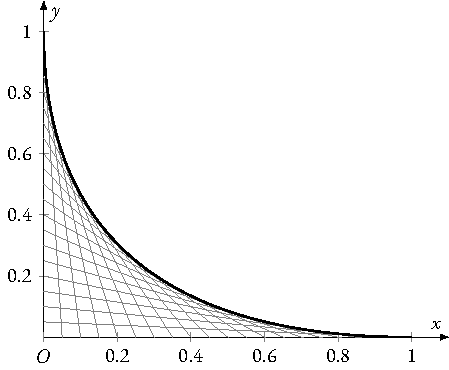
\includegraphics{envelope.pdf}
\end{center}

假如有这样一些直线,它的 \(y\)轴截距和 \(x\)轴截距加起来是 1,并且那两个截距都大于零,图中画出了一些这样的直线(灰色部分),那么黑色曲线就是它的包络线。

琪露诺:哇,好像它就是把灰色线的运动紧紧包裹住了一样。

朱鹭子:差不多,不过实际上应该是相切吧(笑),比如离原点距离为1的直线的包络就是单位圆嘛。

琪露诺:那包络线怎么求呢?

朱鹭子:实际上我们知道那些通解,或者更广泛地,曲线族的形式可以表示为:
\[
	F(t,x,c_1)=0
	.\]

那么包络线的方程是会满足:
\[
	\begin{cases}\\[-2em]
		F(t,x,c_1) =0, \\
		\dfrac{\uppartial F}{\uppartial c_1}=0.
	\end{cases}\tag{E}
\]

针对 \(c_1\)的参数方程。但是满足这方程的曲线可能有很多,其中并不一定有包络线。但毫无疑问的是,包络线的确是一种特殊的存在。现在我们来看看包络线和微分方程的关系:

想想看,对于一个一阶微分方程,它对解曲线的性质描述只精确到一阶导数,那么看看我们的包络线——每一点都有一条曲线族中的曲线\textbf{与之相切},如果这族曲线是一个一阶ODE的解的话……

琪露诺:那是不是意味着,这个包络上面所有点都满足那个方程……因为导数一样了, 点也在那些解的曲线上面。

朱鹭子:没错!这其实就是说这个包络线也是ODE的解,这其实是ODE的\textbf{奇解}。当然这也就意味着不满足那个唯一性条件了,所以根据你之前说的……

琪露诺:隐函数存在定理。

朱鹭子:对,所以对于初始条件 \(x(t_0)=x_0\),应当有:
\[
	\dfrac{\uppartial F(t,x,x')}{\uppartial x'}\Bigg|_{(t_0,x_0)}
	.\]

但这只是最基本的条件,事实上,由E式子我们知道,我们把 \(\dx\) 看成是 \(c_1\)……然后实际上这个\ruby[g]{包络}{奇解}应该满足:
\[
	\begin{cases}\\[-2em]
		F(t,x,x')=0 , \\
		\dfrac{\uppartial F}{\uppartial x'}=0.
	\end{cases}
\]

将这玩意把 \(x'\)消去就是包络线要满足的方程了,同理,这只是其中一个条件而已。

琪露诺:又来……全都是仅仅能满足的程度吗?有没有充要条件呢?

朱鹭子:饶了我吧,我暂时还不知道(笑),上面这个主要是来判断一个ODE有没有奇解的,这样的解往往会……就像幻想乡对于外界一样吧(笑)。

琪露诺:又是听不懂的比喻……

朱鹭子:这倒是有个出名的例子,叫做Clairaut微分方程:
\[
	x=t\dx+f\left( \dx\tag{ſ} \right)
	.\]

琪露诺:这是什么奇怪的记号……积分号吗?

朱鹭子:这个不管,你试试鼓捣鼓捣这个ODE。

琪露诺:哦……首先两边对 \(t\)求导,得到:
\[
	\dx=x\symscr{D} ^2_t(x)+\dx+f'\left( \dx \right)\symscr{D} ^2_t(x)
	.\]

约去两边的 \(\dx\)得到:
\[
	\symscr{D} ^2_t(x)\left( x+f'\left( \dx \right)  \right) =0
	.\]

所以事实上是 \(\symscr{D} ^2_t(x)=0\implies \dx=c_1\)和 \(x+f'\left( \dx \right)=0 \)。

接下来我只需要积分就可以……哦直接代方程……就可以:
\[
	x=c_1x+f(c_1)
	.\]

哇是一坨子直线。所以你的意思是说另外一个 \(x+f'\left( \dx \right)=0\)其实是这些直线的包络吗?

朱鹭子:事实上的确是这样,在这里就先不验证了,但不管怎么样,记住有奇解存在这件事还是相当重要的。


\section{高阶线性微分方程}

\subsection{高阶线性微分方程的解的结构}
朱鹭子:这里我们算是基本把一阶ODE的方法讨论得差不多了,接下来是有关高阶线性微分方程的一些理论。

琪露诺:听上去非常恐怖的样子……

朱鹭子:事实上的确比一般的一阶微分方程要麻烦不少:
\[
	\symscr{L} (x)= f(t)
	.\]

其中,我们认为 \(\symscr{L} \)是一个线性算子,就像之前提到的一样。接下来我们来考虑下最基本的齐次方程:
\[
	\symscr{L} (x)=0\tag{HOMs}\label{HOMs}
	.\]

我们来研究它解的结构。首先,如果(假如有的话) \(x_1(t),\cdots x_k(t)\) 都是它的解,那么这个呢:
\[
	x_{\rm new}= \sum_{i=1}^{k} c_i x_i
	.\]

实际上就是 \(x_1(t),\cdots x_k(t)\) 的线性组合,这个是不是ODE的解呢?

琪露诺:按感觉来说应该是……

朱鹭子:实际上我们可以这样子:

\[
	\symscr{L} \left( \sum_{i=1}^{k} c_i x_i \right) =\sum_{i=1}^{k}\symscr{L}\left(  c_i x_i\right) =\sum_{i=1}^{k} c_i\underset{0}{\underbrace{\symscr{L}\left(  x_i\right)}}=0\label{djyl}
	.\]

上面的等号分别用到了 \(\symscr{L} \)算子的\hyperref[linearofl]{\underline{函数线性}}的两个方面。这实际上被称为\textbf{叠加原理}。

琪露诺:\emoji{😅}

朱鹭子:?

琪露诺:啊没……\emoji{🥶}

朱鹭子:用正常的话来说,就是\(x_1(t),\cdots x_k(t)\)的\textbf{张成}也属于原方程\hyperref[HOMs]{\underline{(HOMs)}}的解空间。而接下来我们需要一个可以衡量这些函数是否线性相关的工具。

琪露诺:为什么要研究他们是不是线性相关的啊……

朱鹭子:因为如果有线性相关的话,证明这些函数之间并不是真正独立的,有些函数可以用其他函数表示。这就意味着你所得到的并不是 \(k\)个解。

琪露诺:原来如此,所以是要用行列式还是什么吗?

朱鹭子:确实可以用行列式,首先看下针对函数的的线性相关/无关:
\begin{itemize}
	\item 如果存在不全为 0 的常数 \(c_1,\cdots ,c_k\),以及函数 \(x_1(t),\cdots x_k(t)\) 使得:
	      \[
		      \sum_{i=1}^{k} c_i x_i(t)\equiv 0
		      .\]
	      在 \(t \in\symcal I\)上面恒成立,这意味着这些函数在区间 \(\symcal{I} \) 上线性相关,否则就是线性无关。
\end{itemize}

实际上就是把线性相关的容差扩展到区间上来(大致来说)。

琪露诺:看起来很之前的线性相关一样。

朱鹭子:但实际上是不一样的。同样,我们可以用行列式的值是否为0来判断(实际上不能)一坨东西是不是真的线性相关,比如Wronsky行列式:
\[
	\symscr{W}_t \left( x_1,\cdots x_k \right) \coloneq \begin{vmatrix}
		x_1(t)         & x_2(t)         & \cdots & x_k(t)         \\
		x_1'(t)        & x_2'(t)        & \cdots & x_k'(t)        \\
		\vdots         & \vdots         &        & \vdots         \\
		x_1^{(k-1)}(t) & x_2^{(k-1)}(t) & \cdots & x_k^{(k-1)}(t) \\
	\end{vmatrix}
	.\]

琪露诺:诶?为什么和求导有关系?

朱鹭子:因为如果线性相关那坨方程: \(\sum_{i=1}^{k} c_i x_i(t)\equiv 0\) ,那么左右两边求导亦为0,这就意味着不管是 \(c_i(t)\) 的多少阶导都是线性相关的(当然建立在可以导那么多次的情况下),实际上是给这些函数一些条件,让他们刚好可以凑成一对行列式。
不管如何,这个行列式可以在某种程度上反应函数是否是线性相关的。
事实上有以下这些定理:
\begin{itemize}
	\item 如果函数们线性相关,那么她们的Wronsky行列式为0。

	      这个其实可以轻易得到存在一组非0的常数 \(C_1,\cdots C_n\) 使得:
	      \[
		      \sum_{i=1}^{k} C_i(t)x_i(t)=0\xlongequal[]{\mbox{\tiny 连续求导 \(k\) 次}} \begin{bmatrix}
			      \sum_{i=1}^{k} C_i x_i(t) \\    \sum_{i=1k}^{k} C_i x_i'(t) \\    \vdots \\    \sum_{i=1}^{k} C_i x^{(k-1)}(t) \\\end{bmatrix}
		      \equiv \symbf 0 \implies\symbfscr{W} \cdot\symbfit C \equiv\symbf 0
		      .\]

	      其中我们不妨设 \(\symbfscr{W}\) 是Wronsky矩阵(即Wronsky行列式去掉行列式符号的形式),而 \(\symbfit C \) 是一个系数矩阵 \(\begin{bmatrix}
		      C_1 &    C_2 &  \cdots  &    C_k \end{bmatrix}^{\rm T}\),我们知道 \(\symbfit C\) 是有非零解的,这意味着 \(\symscr{W} \equiv 0\).
	      另外要指出的事情是,其逆定理一般是不成立的,举个例子吧:\(1,t,\cdots t^{k-1},\symrm{e} ^{-1 / t^2 }\),这一些函数,注意到当 \(t=0\)时,\(\symrm{e} ^{-1 / x^2 }\)的每一阶导都为零,所以此时Wronsky行列式必然有一列全是0,此时行列式为0,但实际上这个函数序列是线性无关的。
	\item 另外一个同样重要的是,如果 \(x_1,\cdots, x_k\) 都是方程 \(\symscr{L} (x)=0\) 的解,那么上面这个“逆定理”反而是成立的。实际上我们可以用的除了刚才那些,还有由于这些函数是ODE的解而使用的存在唯一性定理。
\end{itemize}

琪露诺:为什么这里满足存在唯一性定理的条件呢?

朱鹭子:这里会涉及到高阶微分方程的解的存在唯一性,事实上我们可以把它变成 \(n\) 个一阶线性方程,实际上就是一个线性方程组,具体的存在唯一性这里不再阐述。暂且解决完这个之后,我们继续:
\begin{itemize}
	\item ……另外一个同样重要的是,如果 \(x_1,\cdots, x_k\) 都是方程 \(\symscr{L} (x)=0\) 的解,那么上面这个“逆定理”反而是成立的。实际上我们可以用的除了刚才那些,还有由于这些函数是ODE的解而使用的存在唯一性定理。
	      事实上,这个所谓逆定理指的是:如果 \(x_1,\cdots, x_k\) 都是方程 \(\symscr{L} (x)=0\) 的解且在 \(t \in\symcal{I} \) 上面线性无关,则 \(\symscr{W}_t \left( x_1,\cdots x_k \right)\neq 0,\,\forall t\in\symcal{I} \)。我们可以采用反证法,如果真的有这么一个 \(t_0\) 存在,使得 \(\symscr{W}_t \left( x_1,\cdots x_k \right)\big|_{t_0} \coloneq \symscr{W}( t_0 ) =0 \),那么事实上考虑这样的方程组:
	      \[
		      \symbfscr{W}\left( t_0 \right) \cdot \symbfit C \equiv 0
		      .\]
	      注意这只是针对 \(t_0\) 一个点的方程,由于 \(\symscr{W}( t_0 ) =0\),上面这个方程必然有非零解 \(C_1,\cdots ,C_k\),则考虑下面这个函数:
	      \[
		      x_{\rm add}(t)=\sum_{i=1}^{k} C_i x_i(t),\, t\in\symcal{I} \label{gouzaoofxadd}
		      .\]

	      由于\hyperref[dlyl]{\underline{叠加原理}},\(x_{\rm add}(t)=\)是方程\hyperref[HOMs]{\underline{(HOMs)}}的解。那它满足的初始条件是什么呢?
\end{itemize}

琪露诺:诶?为什么要考察初始条件,这不就一个普通的叠加吗?

朱鹭子:你得想清楚我们这些 \(C_1,\cdots ,C_k\)是怎么来的。

琪露诺:\(\symbfscr{W}\left( t_0 \right) \cdot \symbfit C \equiv= 0\) 的解?那就意味着……
\[
	\begin{bmatrix}
		\sum_{i=1}^{k} C_i x_i(t_0) \\    \sum_{i=1k}^{k} C_i x_i'(t_0) \\    \vdots \\    \sum_{i=1}^{k} C_i x^{(k-1)}(t_0) \\\end{bmatrix}
	\equiv \symbf 0 \implies \sum_{i=1}^{k} C_i x_i^{(m)}(t_0)\equiv 0,\,m=0,1,\cdots k-1
	.\]

这个是什么初始条件……

朱鹭子:你想想这个初始条件是足够确定唯一解的吗?

琪露诺:诶?你这话是什么意思哇,这不全都是写确定的函数 \(x_1,\cdots, x_k\) 吗?

朱鹭子:我们要讨论的可不是这个。事实上,这些初值条件实际上等价于:
\[
	\symscr{D} ^i_t(x_{\rm add}(t))\equiv 0,\,i=0,1,\cdots k-1
	.\]

刚好 \(k\) 个,事实上对于一个 \(k\) 阶方程,这 \(k\) 个初始条件足以确定一个唯一解,那么实际上我们可以认为 \(x_{\rm add}(t)\) 是一个 \(k\) 解ODE的\textbf{唯一}解。你意识到什么问题没有?

琪露诺:啊?没什么问题哇,类比一阶微分方程的结论,这确实是一个有 \(k\) 个初始条件决定的唯一解。

朱鹭子:不是,你看看初始条件都是些什么吧。

琪露诺:全是0?

朱鹭子:对,这实际上意味着这是一个零向量……

琪露诺:哦哦哦所以实际上 \(x\equiv 0\) 也是一个解,然后因为解唯一,所以 \(x_{\rm add}\equiv 0\)。

朱鹭子:没错,然后捏?

琪露诺:\emoji{😨}

朱鹭子:注意到我们是怎么样\hyperref[gouzaoofxadd]{\underline{(构造)}} \(x_{\rm add}\) 的:
\[
	x_{\rm add}(t)=\sum_{i=1}^{k} C_i x_i(t),\, t\in\symcal{I}
	.\]

这意味着
\[
	\sum_{i=1}^{k} C_i x_i(t)\equiv 0
	.\]

琪露诺:哦哦然而事实上根本不可能有这件是存在吧,由于 \(C_1,\cdots ,C_k\)不全为零,这意味着 \(x_1,\cdots x_k\)线性相关了!

朱鹭子:确实,但一开始我们就认为 \(x_1,\cdots x_k\) 是线性无关的,因此导出了矛盾,所以
\[
	\symscr{W}_t \left( x_1,\cdots x_k \right) \neq 0,\,\forall t\in\symcal{I}
	.\]

这个是成立的。在刚才的讨论中,我们意识到对于这样的Wronsky矩阵,在某一点处为0就可以推出定义域上的函数值都是0。

琪露诺:这是为什么哇?

朱鹭子:这个嘛……你可以去问问那个九尾妖狐,在这里(喝水)没什么时间说这个。好,我们知道了大致有关Wronsky行列式的两个结论,在这里总结一下:
\begin{itemize}
	\item 如果 \(x_1,\cdots x_k\) 在 \(\symcal{I} \)线性相关,则在 \(\symcal{I} \) 上Wronsky行列式恒为零。
	\item 如果\(x_1,\cdots x_k\) 是方程 \(\symscr{L} (x)=0\) 的解,且在 \(\symcal{I} \)线性无关,则在 \(\symcal{I} \) 上Wronsky行列式恒不为零。
\end{itemize}

事实上第一个可以等价于:
\[
	\boxed{\mbox{如果只要有一点 \(t_0\) 对应的 Wronsky 行列式不为零,则\(x_1,\cdots x_k\)线性无关。}}
\]

琪露诺:这不就是逆否命题吗?

朱鹭子:有用的,我们继续,接下来对于一个 \(n\) 解的线性方程,我们总是可以找到它的 \(n\) 个解,线性相关也能接受,然后给出 \(n\) 个初始条件,这些初始条件我们可以任意选取。

琪露诺:为什么哇?

朱鹭子:因为首先,存在唯一性定理保证这个初始条件对应的解必然存在且唯一,此时我们要验证的其实是上面 \(n\) 个解线性无关的情况存在,为了保证这样,我们需要看一下盒子里的内容,保证Wronsky 行列式至少有一点不为零,实际上这一点就对应了初始条件。看,如果Wronsky 行列式长这样:
\[
	\symscr{W} (t_0)=\begin{vmatrix}
		1      & 0      & \cdots & 0      \\
		0      & 1      & \cdots & 0      \\
		\vdots & \vdots &        & \vdots \\
		0      & 0      & \cdots & 1      \\
	\end{vmatrix}=1
	.\]

实际上对应了初始条件。

琪露诺:为什么要是这样一个对角阵呢?

朱鹭子:只是让他不为0罢了,实际上这个行列式对应了初始条件:
\[
	\begin{bmatrix}
		x_1(t_0) & x_1'(t_0) & \cdots & x_1^{(n-1)}(t_0) \\
		x_2(t_0) & x_2'(t_0) & \cdots & x^{(n-1)}_2(t_0) \\
		\vdots   & \vdots    &        & \vdots           \\
		x_n(t_0) & x_n'(t_0) & \cdots & x_n^{(n-1)}(t_0) \\
	\end{bmatrix}=\begin{bmatrix}
		1      & 0      & \cdots & 0      \\
		0      & 1      & \cdots & 0      \\
		\vdots & \vdots &        & \vdots \\
		0      & 0      & \cdots & 1      \\
	\end{bmatrix}
	.\]

这个实际上对应了 \(n\) 组初始条件,每组条件对应一个解 \(x_i(t)\),由于存在唯一性定理,这些解 \(x_1,\cdots ,x_n\)必然存在,而且她们对应的 Wronsky 行列式在 \(t=t_0\) 处不为0,这就意味着这实际上是 \(n\) 阶方程的 \(n\) 个线性无关解。

琪露诺:但是实际上 \(n\) 阶方程最多也有 \(n\) 个解吧?

朱鹭子:线性方程, \(n\) 阶线性方程的通解最多只有 \(n\) 个独立参数,这所谓的通解可以表示为:
\[
	x_{\rm G}=\sum_{i=1}^{n} c_i x_i
	.\]

其中 \(x_i\) 是方程的一组线性无关解。这意味着一个 \(n\) 阶齐次线性ODE\textbf{必然}有 \(n\) 个线性无关的解。这被称为该ODE的基本解组。

琪露诺:但这只是齐次的呀,如果不是齐次的话怎么找积分因子呢?

朱鹭子:你总不会认为 \(n\) 阶线性还得靠找积分因子来求非齐次方程的解吧?

琪露诺:那不是……那难道是什么?猜吗?

朱鹭子:猜……倒是的确有这种,不过这里暂且先不论。这里主要讨论的是常数变易法。


\subsection{高阶线性微分方程与常数变易法}
琪露诺:\emoji{😥},细说。

朱鹭子:呃……其实就是把 \(c_1,\cdots ,c_n\) 这些常数全部变成函数。

琪露诺:诶?这么做有根据吗?

朱鹭子:对线性方程来说,可以用唯一性定理。实际上,常数变易其实是利用了齐次和非齐次之间的关系,比如:
\[
	c_1(t)x_1(t)
	.\]

我求导完之后就是:
\[
	c_1'(t)x_1(t)+c_1(t)x_1'(t)
	.\]

实际上上面两个可以分别对应方程的齐次部分和非齐次部分。

琪露诺:呜呜……还是很抽象……

朱鹭子:那让我们看一个具体的例子:

\begin{tho}{高阶非齐次线性微分方程的常数变易解法}
	在\textbf{已经知道基本解组} \(x_1(t),\cdots x_n(t)\)的情况下, \(n\)阶微分方程  \(\symscr{L} (x)=f(t)\)的所有解可以表示成如下形式:
	% \[
	% 	x_{\rm All}= \sum_{i=1}^{n} x_i(t) \, \cdot \int 	\dfrac{\scriptstyle	\begin{vNiceMatrix}[first-row,columns-width = 0.1cm,cell-space-limits = 1pt]\renewcommand{\arraycolsep}{0pt}
	% 			                                 &                             &                     & \raisebox{-1ex}{$\!\!\!\!\!\scriptscriptstyle k-{\rm column}\!\!\!\!\!\!\!$} &                     &                             \\
	% 			\scriptstyle \scriptstyle x_1(t) & \scriptstyle x_2(t)         & \scriptstyle \cdots & \scriptstyle 0                                & \scriptstyle \cdots & \scriptstyle x_n(t)         \\[-3pt]
	% 			\scriptstyle x_1'(t)             & \scriptstyle x_2'(t)        & \scriptstyle \cdots & \scriptstyle 0                                & \scriptstyle \cdots & \scriptstyle x_n'(t)        \\[-3pt]
	% 			\scriptstyle \vdots              & \scriptstyle \vdots         & \scriptstyle \cdots & \scriptstyle \vdots                           & \scriptstyle \cdots & \scriptstyle \vdots         \\[-3pt]
	% 		\scriptstyle x_1^{(n-1)}(t)     &\!\! \!\scriptstyle x_n^{(n-1)}(t) \!\!\!& \scriptstyle \cdots & \scriptstyle 1                                & \scriptstyle \cdots &\!\! \!\scriptstyle x_n^{(n-1)}(t) \!\!\\
	% 		\end{vNiceMatrix}}{\symscr{W} (t)}f(t) \,\mathrm{d}t
	% 	.\]
	\[
		x_{\rm Sol}= \sum_{i=1}^{n} x_i(t) \, \cdot \int\left(  \raisebox{-2.5em}{\(\dfrac{{
			\begin{vmatrix}
				\scriptstyle x_1(t)         & \scriptstyle x_2(t)                       & \scriptstyle \cdots & \scriptstyle 0      & \scriptstyle \cdots & \scriptstyle x_n(t)                     \\[-3pt]
				\scriptstyle x_1'(t)        & \scriptstyle x_2'(t)                      & \scriptstyle \cdots & \scriptstyle 0      & \scriptstyle \cdots & \scriptstyle x_n'(t)                    \\[-3pt]
				\scriptstyle \vdots         & \scriptstyle \vdots                       & \scriptstyle \cdots & \scriptstyle \vdots & \scriptstyle \cdots & \scriptstyle \vdots                     \\[-3pt]
				\scriptstyle x_1^{(n-1)}(t) & \!\! \!\scriptstyle x_n^{(n-1)}(t) \!\!\! & \scriptstyle \cdots & \scriptstyle 1      & \scriptstyle \cdots & \!\! \!\scriptstyle x_n^{(n-1)}(t) \!\! \\[3pt]
			\end{vmatrix}\kern-4em\raisebox{1.8em}{$\kern-8em\overset{i}{\overbrace{\phantom{zzxvxvxvxx3wixcb}}}$\kern 4.6em}}}{\symscr{W} (t)}\)}f(t) \right) \,\mathrm{d}t
		.\]
\end{tho}

琪露诺:\emoji{😅}
\emoji{😅}
\emoji{😅}
\emoji{😅}
\emoji{😅}
\emoji{😅}
\emoji{😅}
\emoji{😅}
\emoji{😅}
\emoji{😅}
\emoji{😅}
\emoji{😅}
\emoji{😅}
\emoji{😅}
\emoji{😅}
\emoji{😅}
\emoji{😅}
\emoji{😅}
\emoji{😅}
\emoji{😅}
\emoji{😅}
\emoji{😅}
\emoji{😅}
\emoji{😅}
\emoji{😅}
\emoji{😅}
\emoji{😅}
\emoji{😅}
\emoji{😅}
\emoji{😅}
\emoji{😅}
\emoji{😅}
\emoji{😅}
\emoji{😅}
\emoji{😅}
\emoji{😅}
\emoji{😅}
\emoji{😅}
\emoji{😅}
\emoji{😅}
\emoji{😅}
\emoji{😅}
\emoji{😅}
\emoji{😅}
\emoji{😅}
\emoji{😅}
\emoji{😅}
\emoji{😅}
\emoji{😅}
\emoji{😅}
\emoji{😅}
\emoji{😅}


% \[\mbox{\Huge\emoji{😅}}
% \begin{matrix}
% 	\mbox{\emoji{😅}} & \mbox{\emoji{😅}} & \mbox{\emoji{😅}} \\
% 	\mbox{\emoji{😅}} & \mbox{\emoji{😅}} & \mbox{\emoji{😅}} \\
% 	\mbox{\emoji{😅}} & \mbox{\emoji{😅}} & \mbox{\emoji{😅}} \\
% \end{matrix}\mbox{\Huge\emoji{😅}}
% \]
这又是那么多行列式的……这哪里能算?\emoji{😅}

朱鹭子:本身就是不是专门来要你算的啊,而且你没有注意到这个可以机械地给出所有解吗?这比什么取巧的猜测证明要通用的多了。

琪露诺:是倒是……不过当初人们是怎想到用行列式去解决这些破问题的呢?

朱鹭子:其实根本上还是常数变易法,之前我就和你说要记住这个了。

琪露诺:诶?

朱鹭子:这样吧,我给你大概说下,本身我们是知道对于一个线性微分方程 \(\symscr{L} (x)=0\) ,在已知其基本解组 \(x_i\)的情况下,我们可以认为它的所有解如下:
\[
	x_{\rm All,\ HOM} = \sum_{i=1}^{n} c_i x_i(t)
	.\]

指的其实就是其线性组合,现在我们应用常数变易法,\textbf{假设}这样一个非齐次的线性方程的解是:
\[
	x_{\rm Sol} \coloneq \sum_{i=1}^{n} c_i(t) x_i(t)
	.\]

好,但是这样有个问题——琪露诺!你来回答,出了什么问题?

琪露诺:我怎么可能知道……你仅仅是变易了一下就出问题了?

朱鹭子:事实上,常数变易本身是没有问题的,但是真正出问题的时候,我们现在只有:
\[
	\symscr{L} (x_{\rm Sol}) = \symscr{L} \left( \sum_{i=1}^{n} c_i(t)x_i(t) \right) =0
	.\]

这一条方程,但是我们要求的是……

琪露诺:所有的\(c_i(t)\)?

朱鹭子:对,所以方程数量是不够的,那怎么办?

琪露诺:这不挺好的吗,这样找解就方便多了。

朱鹭子:的确,但是怎么找呢?我们知道这样的 \(c_i(t)\) 必有无穷组,他们之间又有什么关系呢?

琪露诺:不清楚……

朱鹭子:事实上这是一个线性方程,如果我们等价到线性代数里面去的话,那么事实上我们可以给出另外 \(n-1\) 个方程来给出,凑够 \(n\) 个方程之后反倒会给出个比较容易看得出来的解。那么给出的这些方程需要满足什么条件捏?

琪露诺:线性?

朱鹭子:没错,针对哪些线性?

琪露诺:那应该是针对 \(c_i(t)\) 和 \(x_i(t)\) 线性就可以了吧……

朱鹭子:我给一个,你看看:
\[
	\sum_{i=1}^{n}\symscr{D} _t(x_i)\cdot \symscr{D} _t(c_i)=0
	.\]

是线性的吗?

琪露诺:是,因为求导运算和乘法本身就是线性的,所以这个方程分别对 \(c_i(t)\) 和 \(x_i(t)\) 线性。

朱鹭子:没错。

琪露诺:那为什么要给这个呢?

朱鹭子:是为了方便计算,且听我说。我们看看刚才的 \(x_{\rm Sol}=\sum_{i=1}^{n} c_i(t)x_i(t)\),左右两边求导得到:
\[
	\symscr{D} _t\left( x_{\rm Sol} \right) = \sum_{i=1}^{n}\left(  \symscr{D} _t(c_i)x_i+\symscr{D} _t(x_i)c_i\right)  =\underset{0}{\underbrace{ \sum_{i=1}^{n}\symscr{D} _t(c_i)x_i}}+\sum_{i=1}^{n}\symscr{D} _t(x_i)c_i=\sum_{i=1}^{n}\symscr{D} _t(x_i)c_i
	.\]

看!这样我们实际上就简化了 \(\symscr{D} _t\left( x_{\rm Sol} \right) \),只通过一次条件,另外,我问一下为什么我要消去这个 \(\sum_{i=1}^{n}\symscr{D} _t(c_i)x_i\) 而不是 \(\sum_{i=1}^{n}\symscr{D} _t(x_i)c_i\)?

琪露诺:\emoji{🤔}……也许是因为 \(x_i\) 是 \(\symscr{L} (x)=0\) 的解?

朱鹭子:对,继续。

琪露诺:说不出来了……

朱鹭子:事实上,是为了保持求导次数一致,我们知道 \(\symscr{L} \) 的表示是:
\[
	\symscr{D} ^n+\sum_{i=1}^{n-1} a_i(t)\symscr{D} _t^i
	.\]

观察到不同阶导前面乘上的函数是不一样的,然而我们要保持 \(\symscr{D} ^n(x_i)+\sum_{i=1}^{n-1} a_i(t)\symscr{D} _t^i (x_i) = 0\) 这个良好的性质,我们需要让 \(\symscr{D} _t^k(x_{\rm Sol})\) 应该对应 \(\symscr{D} _t^k(x_i)\) ,这样子的话,包含所有这些 \(x_i\) 的到时候可以消掉。我们继续,我们现在知道了:
\[
	\symscr{D} _t\left( x_{\rm Sol} \right) =\sum_{i=1}^{n}\symscr{D} _t(x_i)c_i
	.\]

我们继续求导顺便再给出一个条件:
\[
	\symscr{D}^2 _t\left( x_{\rm Sol} \right) =\sum_{i=1}^{n}\symscr{D}^2 _t(x_i)c_i+\underset{\mbox{\tiny 令这个为零}}{\underbrace{\sum_{i=1}^{n}\symscr{D} _t(c_i)\symscr{D} _t(x_i)}}=\sum_{i=1}^{n}\symscr{D}^2 _t(x_i)c_i
	.\]

琪露诺:哇,和第一次求导的时候长得差不多。

朱鹭子:没错,事实上我可以一直这样做,直到我用完了 \(n-1\) 个条件:只要带上 \(\symscr{D} _t(c_i)\) 的求和就让他为零,这样我就可以保证对 \(x_{\rm Sol}\) 的导数阶数和对 \(x_i\) 的导数阶数相等,因此我给出的 \(n-1\) 个条件和推论应该是:
\[
	\begin{bmatrix}
		\sum_{i=1}^{n} \symscr{D} _t(c_i)x_i \\    \sum_{i=1}^{n} \symscr{D} _t(c_i)\symscr{D} _t(x_i) \\    \vdots \\    \sum_{i=1}^{n} \symscr{D} _t(c_i)\symscr{D}^{n-2} _t(x_i) \\\end{bmatrix}=\symbf 0 \implies \begin{bmatrix}
		\symscr{D} _t(x_{\rm Sol}) \\ \symscr{D} ^2_t(x_{\rm Sol})    \\   \vdots  \\    \symscr{D} _t^{n-1}(x_{\rm Sol}) \\\end{bmatrix}=\begin{bmatrix}
		\sum_{i=1}^{n}\symscr{D} _t(x_i)c_i \\    \sum_{i=1}^{n} \symscr{D} _t^2(x_i)c_i \\    \vdots \\  \sum_{i=1}^{n} \symscr{D} _t^{n_-1}(x_i)c_i   \\\end{bmatrix}
	.\]
接下来,我把他带进 \(\symscr{L} (x_{\rm Sol})=\symscr{D} _t^n(x_{\rm Sol})+ \sum_{i=1}^{n-1} a_i(t)\symscr{D} _t^i(x_{\rm Sol})\),你就能发现我们是怎么对付“求导”这个最大的不稳定因素的:
\[
	\symscr{L} (x_{\rm Sol}) =\symscr{D} _t^n(x_{\rm Sol}) +\sum_{i=1}^{n-1} a_i(t)\symscr{D} _t^i(x_{\rm Sol}) =\symscr{D} _t\left(  \symscr{D} _t^{n-1}(x_{\rm Sol}) \right) + \sum_{i=1}^{n} a_i(t)
	\sum_{j=1}^{n} c_j\symscr{D} _t^j(x_j)\tag{$\mathrm{SOL}^n$}
	.\]

琪露诺:看起来非常复杂……虽然你只是把所有东西都代进去而已,但是这个二重求和……

朱鹭子:确实,但是在这里我们可以先互换啊\emoji{😀}:
\[
	\begin{aligned}
		(\mathrm{SOL}^n) & = \underset{\symscr{D} _t\left(\sum_{j=1}^{n} \symscr{D} _t^{n_-1}(x_j)c_j   \right) \,=\, \sum_{j=1}^{n}\symscr{D} ^n_t(x_j)c_j+\symscr{D} _t^{n-1}(x_j)\symscr{D} (c_j)}{\underbrace{\symscr{D} _t\left(  \symscr{D} _t^{n-1}(x_{\rm Sol}) \right)}} + \sum_{i=1}^{n} a_i(t)
		\sum_{j=1}^{n} c_j\symscr{D} _t^j(x_j)                                                                                                                                                                                                                                                               \\
		                 & =\sum_{j=1}^{n}\symscr{D} ^n_t(x_j)c_j+\symscr{D} _t^{n-1}(x_j)\symscr{D}_t (c_j)+\sum_{j=1}^{n} c_j\sum_{i=1}^{n} a_i(t)
		\symscr{D} _t^j(x_j)                                                                                                                                                                                                                                                                                 \\
		                 & =\underset{\sum_{j=1}^{n} c_j\symscr{L} (x_j)=0}{\underbrace{\sum_{j=1}^{n} c_j\left( \symscr{D} _t^n(x_j)+\sum_{i=1}^{n} a_i(t)\symscr{D} _t^i(x_j) \right)}}+\sum_{j=1}^{n}\symscr{D} _t^{n-1}(x_j)\symscr{D} _t(c_j)=\sum_{j=1}^{n}\symscr{D} _t^{n-1}(x_j)\symscr{D} _t(c_j).
	\end{aligned}
\]

琪露诺:\emoji{😪😪😪😪😪}

朱鹭子:别担心,虽然看起来很复杂,但最后的结果其实相当简单啊:
\[
	\symscr{L} (x_{\rm Sol})=\sum_{j=1}^{n}\symscr{D} _t^{n-1}(x_j)\symscr{D} _t(c_j) =f(t)
	.\]

琪露诺:那这有什么用呢?

朱鹭子:看,我们刚才给出了 \(n-1\) 个方程,但实际上我们要解出 \(c_i\) 必然还需要一个,而 \(x_{\rm Sol}=\sum_{i=1}^{n} x_i(t) c_i(t)\) 并不能算解出 \(c_i\) 的方程,因为我们本身就要解出 \(c_i\) 才知道 \(x_{\rm Sol}\) 的,而这 \(\sum_{j=1}^{n}\symscr{D} _t^{n-1}(x_j)\symscr{D} _t(c_j) =f(t)\)就是最后的方程,如果把这个方程和我们写出来的那 \(n-1\)方程一起写出来:
\[
	\begin{bmatrix}
		\sum_{i=1}^{n} \symscr{D} _t(c_i)x_i \\    \sum_{i=1}^{n} \symscr{D} _t(c_i)\symscr{D} _t(x_i) \\    \vdots \\    \sum_{i=1}^{n} \symscr{D} _t(c_i)\symscr{D}^{(n-2)} _t(x_i) \\
		\sum_{i=1}^{n} \symscr{D} _t(c_i)\symscr{D}^{(n-1)} _t(x_i)
	\end{bmatrix}= \begin{bmatrix}
		0 \\    0 \\    \vdots \\    0 \\    f(t) \\\end{bmatrix}
	.\]

看到这个你想到了什么没有,尤其是左边矩阵里面这个求和?

琪露诺:看起来……是矩阵相乘?

朱鹭子:没错确实是矩阵相乘,实际上:
\[
	\begin{bmatrix}
		\sum_{i=1}^{n} \symscr{D} _t(c_i)x_i \\    \sum_{i=1}^{n} \symscr{D} _t(c_i)\symscr{D} _t(x_i) \\    \vdots \\    \sum_{i=1}^{n} \symscr{D} _t(c_i)\symscr{D}^{(n-2)} _t(x_i) \\
		\sum_{i=1}^{n} \symscr{D} _t(c_i)\symscr{D}^{(n-1)} _t(x_i)
	\end{bmatrix}= \underset{\symbfscr W(t)}{\underbrace{\begin{bmatrix}
		x_1                & x_2                & \cdots & x_n                \\
		\symscr{D} _t(x_1) & \symscr{D} _t(x_2) & \cdots & \symscr{D} _t(x_n) \\
		\vdots             & \vdots             &        & \vdots             \\
		\symscr{D}^{n-1} _t(x_1) & \symscr{D}^{n-1} _t(x_2)     & \cdots & \symscr{D}^{n-1} _t(x_n)     \\
	\end{bmatrix} }}\cdot \begin{bmatrix}
		\symscr{D} _t(c_1) \\   \symscr{D} _t(c_2) \\    \vdots \\    \symscr{D} _t(c_n) \\\end{bmatrix}=\begin{bmatrix}
		0 \\      \vdots \\    0 \\    f(t) \\\end{bmatrix}
	.\]

琪露诺:噢噢噢噢噢噢噢噢哦哦哦哦哦哦哦!!!!!!!!!!!!我懂了!!!所以你的意思是说,由于 \(x_1,\cdots ,x_n\) 一开始就是线性无关的,所以 \(\symbfscr W\) 的行列式必然恒不为零,所以它必然恒有逆!

朱鹭子:在区间 \(\symcal{I} \) 上。没错,所以这样子我们就可以知道:
\[
	\begin{bmatrix}
		\symscr{D} _t(c_1) \\   \symscr{D} _t(c_2) \\    \vdots \\    \symscr{D} _t(c_n) \\\end{bmatrix} = \symbfscr W^{-1}(t)\cdot\begin{bmatrix}
		0 \\      \vdots \\    0 \\    f(t) \\\end{bmatrix}
	.\]

然后观察到 \(f(t)\) 对应的向量只有最后一个元素,因此实际上只有 \( \symbfscr W^{-1}(t)\) 的最后一列是有用的,因此利用Cramer法则(我们求解的是 \( \symscr{D} _t(c_i)\)所以最后还要积分一下)就可以化成:
\[
	x_{\rm Sol}= \sum_{i=1}^{n} x_i(t) \, \cdot \int\left(  \raisebox{-2.5em}{\(\dfrac{{
		\begin{vmatrix}
			\scriptstyle x_1(t)         & \scriptstyle x_2(t)                       & \scriptstyle \cdots & \scriptstyle 0      & \scriptstyle \cdots & \scriptstyle x_n(t)                     \\[-3pt]
			\scriptstyle x_1'(t)        & \scriptstyle x_2'(t)                      & \scriptstyle \cdots & \scriptstyle 0      & \scriptstyle \cdots & \scriptstyle x_n'(t)                    \\[-3pt]
			\scriptstyle \vdots         & \scriptstyle \vdots                       & \scriptstyle \cdots & \scriptstyle \vdots & \scriptstyle \cdots & \scriptstyle \vdots                     \\[-3pt]
			\scriptstyle x_1^{(n-1)}(t) & \!\! \!\scriptstyle x_n^{(n-1)}(t) \!\!\! & \scriptstyle \cdots & \scriptstyle 1      & \scriptstyle \cdots & \!\! \!\scriptstyle x_n^{(n-1)}(t) \!\! \\[3pt]
		\end{vmatrix}\kern-4em\raisebox{1.8em}{$\kern-8em\overset{i}{\overbrace{\phantom{zzxvxvxvxx3wixcb}}}$\kern 4.6em}}}{\symscr{W} (t)}\)}f(t) \right) \,\mathrm{d}t
	.\]

琪露诺:原来是这样……但是感觉无论是对人类还是对妖怪来说计算量都是太大了吧?

朱鹭子:那我们看看二阶的情况?

琪露诺:二阶的话也是代进去嘛,不过倒是有计算可行性:
\[
	x_{\rm Sol}= x_1(t)\int \dfrac{-x_2(t)f(t)}{\symscr{W}(t)}  \,\mathrm{d}t+x_2(t)\int \dfrac{x_1(t)f(t)}{\symscr{W}(t) } \,\mathrm{d}t
	.\]

看起来正常多了,虽然解一个二阶方程用Cramer法则就是有大病。

朱鹭子:但至少能写出来嘛,能写出一条公式出来不是很美妙的事情吗?

琪露诺:\textbf{*不}。而且这种方法要求我们知道基本解组,这要求我们对齐次的方程了如指掌才行。

朱鹭子:确实……求这些一般是很难的……在这里将给出一个比较重要的种类,那就是常系数齐次微分方程。经过之前的讨论,我们知道只要求出线性微分方程的基本解组就能得出其非齐次方程的解,这样子我们只需要考虑基本解组就可以了。

\subsection{常系数线性微分方程的基本解组}

朱鹭子:对于任意一个线性方程,我们不可能得到它的基本解组,但是如果 \(\symscr{L} \) 是不随时间改变而改变的,即 \(\symscr{L} \) 中所有的 \(a_i(t)\) 都是常数,那么这样一个方程我们是很容易得到它的基本解组的。

琪露诺:果然还是只能搞最基本简单的方程啊……

朱鹭子:的确是这样,我们看下面这个方程:
\[
\symscr{L}_c (x)\coloneq\symscr{D} _t^n(x)+ \sum_{i=1}^{n-1} a_i\symscr{D} ^i_t(x)=0
.\]
我们称为常系数线性齐次微分方程。

琪露诺:变成了常数之后应该好搞很多吧?

朱鹭子:是,我们不妨考虑 \( x =\symrm{e} ^{\lambda t}\) 。至于为什么要这么设,实际上是因为对于一阶的:\( \dx+ax=0\) 的解是 \(x= c_1\symrm{e} ^{-at}\) ,所以我们照葫芦画瓢:
\[
	\symscr{L}_c (x) = \symscr{D} _t^n\left( \symrm{e} ^{\lambda t} \right) + \sum_{i=1}^{n-1} a_i\symscr{D} ^i_t\left( \symrm{e} ^{\lambda t} \right) 
	=\left( \lambda ^n+ \sum_{i=1}^{n-1} a_i \lambda ^i \right)\symrm{e} ^{\lambda t}=0\implies \lambda ^n+ \sum_{i=1}^{n-1} a_i \lambda ^i =0
\]

琪露诺:哇!变成最基本的代数方程了!接下来不就是解那个 \(n\) 阶方程就可以了吗?

朱鹭子:实际上也没有这么简单,这个方程被称为常系数线性齐次方程组的特征方程,事实上:
\begin{enumerate}
	\setcounter{enumi}{0}
	\item 如果方程 \(\lambda ^n+ \sum_{i=1}^{n-1} a_i \lambda ^i =0\) 有 \(n\) 个不同的解 \(\lambda_1,\cdots ,\lambda _n \) 那么这个常系数线性齐次分方程的基本解组就是 \( \symrm{e} ^{\lambda _1t},\cdots ,\symrm{e} ^{\lambda_nt}\)。
\end{enumerate}
 
琪露诺:这不是没什么问题吗?

朱鹭子:但实际上,这只是最好的情况,如果特征方程有重根呢?

琪露诺:啊?那也不一样……等等,有重根就意味着实际上这些 \(\symrm{e} ^{\lambda _it}\) 没有 \(n\) 个!那也就是说会有其他解。

朱鹭子:的确,事实上:
\begin{enumerate}
	\setcounter{enumi}{1}
	\item 如果方程 \(\lambda ^n+ \sum_{i=1}^{n-1} a_i \lambda ^i =0\) 有根 \(\lambda _1,\cdots \lambda_k\) 对应重数 \(m_1,\cdots ,m_k\) ,其中 \(\sum_{i=1}^{k} m_i=n\) ,那么这个常系数线性齐次分方程的基本解组就是:
\[
t^j\symrm{e} ^{\lambda_i t},\,j=0,1,\cdots m_i-1,\,i=1,\cdots k
.\]
\end{enumerate}

琪露诺:?这啥,怎么那么多符号,看不懂的啦……

朱鹭子:举个例子,如果特征方程是这样的 \((\lambda -5)^n(\lambda -1)(\lambda -4)^m\) ,那么它对应的常系数线性齐次分方程的基本解组就是:
\[
	\begin{aligned}
	&\symrm{e} ^{5t},t\symrm{e} ^{5t},\cdots t^{n-1}\symrm{e} ^{5t}, \\ 
	&\symrm{e} ^{t},\\
	&\symrm{e} ^{5t},t\symrm{e} ^{4t},\cdots ,t^{m-1}\symrm{e} ^{4t}.
	\end{aligned}
\]

琪露诺:这样下去倒的确是 \(n\) 个线性无关解没错了,但为什么是在前面乘上 \(t^i\)  呢?

朱鹭子:常数变易法\emoji{😂}。实际上这个确实不好怎么说明。

琪露诺:又来\emoji{🤔}……

朱鹭子:不妨只设只有一个重根 \(\lambda_1 \) ,重数为 \(m_1\) ,则用常数变易法设这根对应的解是 \( c(t)\symrm{e} ^{\lambda t}\)。则:
\[
\symscr{D} _t^k (c(t)\symrm{e} ^{\lambda t})=\symrm{e} ^{\lambda t}\sum_{i=0}^{k} \binom{k}{i}\lambda ^i\symscr{D} ^{k-i}_t(c)
.\]

琪露诺:?这是求 \(k\) 阶导?

朱鹭子:是,事实上这是依赖高阶导数的Leibniz公式:
\[
	\symscr{D} _t^k(a\cdot b)= \sum_{i=0}^{k} \binom{k}{i}\symscr{D} ^{k-i}_t(a)\cdot \symscr{D} ^{i}_t(b)
.\]

考虑到这个 \(\sum_{i=0}^{k} \binom{k}{i}\lambda ^i\symscr{D} ^{k-i}_t(c)\)也是常系数线性的,那么实际上:
\[
\begin{aligned}
	\symscr{L} _c(c(t)\symrm{e} ^{\lambda t}) &= \symrm{e} ^{\lambda t}\sum_{i=0}^{n} \binom{n}{i}\lambda ^i\symscr{D} ^{n-i}_t(c)+\sum\limits_{k=1}^{n-1} a_i\symrm{e} ^{\lambda t}\sum_{i=0}^{k} \binom{k}{i}\lambda ^i\symscr{D} ^{k-i}_t(c)\\ 
	&=\symrm{e} ^{\lambda t}\underline{\left( \sum_{i=0}^{n} \binom{n}{i}\lambda ^i\symscr{D} ^{n-i}_t(c)+ \sum\limits_{k=1}^{n-1} a_i\sum_{i=0}^{k} \binom{k}{i}\lambda ^i\symscr{D} ^{k-i}_t(c)\right) }=0.
\end{aligned}
\]

则下划线部分也是常系数线性的,因此不妨设为 \(\overline{\symscr{L} _c}(c)\)。

琪露诺:\emoji{😪😪😪😪😪😪},计算量太大了吧。

朱鹭子:确实,但我们目的不是为了计算,只要是它是常系数线性的就可以,现在已经变成:
\[
\symscr{L} _c(c\cdot\symrm{e} ^{\lambda t}) = \overline{\symscr{L} _c}(c)\symrm{e} ^{\lambda t}=0\implies\overline{\symscr{L} _c}(c)=0
.\]

琪露诺:所以我们要解一个新的常系数线性?

朱鹭子:当然不可能直接解,为了方便讨论,我们不妨设两个线性算符的对应的特征方程为:
\[
\begin{aligned}
	\symscr{L} : \lambda ^n +\sum\limits_{i=1}^{n-1} a_i \lambda ^i\eqcolon A(\lambda ), \\ 
	\overline{\symscr{L}} : \lambda ^n +\sum\limits_{i=1}^{n-1} b_i \lambda ^i\eqcolon B(\lambda ).
\end{aligned}
\]

琪露诺:诶为什么这个超级怪的 \( \overline{\symscr{L} }\) 的 \(n\) 阶导数前面的系数也是 1 呢?

朱鹭子:这个啊,仔细看上面这个方程:
\[
	B(\lambda )=\underline{\sum_{i=0}^{n} \binom{n}{i}\lambda ^i\symscr{D} ^{n-i}_t(c)}+ \sum\limits_{k=1}^{n-1} a_i\sum_{i=0}^{k} \binom{k}{i}\lambda ^i\symscr{D} ^{k-i}_t(c)
.\]

实际上能产生 \(n\) 阶导数的也只有下换线部分吧?你把 \(i=0\)代进去即可,其他看起来很恐怖,但是其实都是常数(只不过很复杂)罢了,这里我们完全可以不考虑。接下来就是线性算符和特征方程之间的关系:
\[
	\symscr{L} (\symrm{e} ^{kx})=A(k)\symrm{e} ^{kx},\,\overline{\symscr{L}} (\symrm{e} ^{kx})=B(k)\symrm{e} ^{kx}
.\]

琪露诺:对,因为 \(\symrm{e} ^{kx}\) 求导不会变,所以完全可以提出来,再加上求导算符乘上的都是常数,所以最后实际上变成了一个 \(\symrm{e} ^{kx}\) 乘上一个固定多项式的情形。

朱鹭子:没错,接下来是重点,要知道我们还有这个哇:
\[
\symscr{L} (c \cdot \symrm{e} ^{kx})=\overline{\symscr{L} }(c)\symrm{e} ^{kx}
.\]

注意到 \(\overline{\symscr{L} }\) 的定义虽然复杂,但实际上并没有和 \(t\) 有关系,也就是说不管是什么样的函数 \(c\) 上式都是满足的。

琪露诺:看起来好像有点形状了……但是我令 \(c=t^i\) 并不能得到什么哇?

朱鹭子:接下来看:
\[
	\symscr{L} ( \symrm{e} ^{k x}\cdot \symrm{e} ^{\lambda x})=\overline{\symscr{L} }(\symrm{e} ^{k x})\symrm{e} ^{\lambda x}=\underline{B(k)\symrm{e} ^{(k+\lambda )x}}
.\]

同时
\[
	\symscr{L} ( \symrm{e} ^{k x}\cdot \symrm{e} ^{\lambda x}) =\underline{ A(\lambda +k)\symrm{e} ^{(k+\lambda )x}}
.\]

注意下划线部分,我们可以得到:
\[
	A(\lambda +k)=B(k)
.\]

琪露诺:哇,所以这就是把这个抽象的多项式表达出来了?

朱鹭子:确实,但是还有哦,之前过了,这个 \(\lambda \) 是多项式 \(A\) 的 \(m\)重根,这意味着:
\[
\symscr{D} _k^i(A(\lambda +k))\bigr|_{k=0} =\symscr{D} _k^i(B(k))\bigr|_{k=0}=0,\,i=0,1,\cdots m-1
.\]

琪露诺:所以是依靠 \(\lambda \) 是 \(A\) 的 \(m\) 重零点来推出这个的吗?

朱鹭子:的确,所以你也看到了, \(0\) 是多项式 \(B(k)\) 的 \(m\) 阶零点,因此?

琪露诺:啊?这不又会到了一开始有多重根的情况了吗?

朱鹭子:看起来好像是这样子,但实际上不一样哦,如果 \(B(k)\) 是这样子的话,那不就意味着 \(B(k)\) 的形式是:
\[
k^n+\sum\limits_{i=m}^{n-1} b_ik^i
.\]

对应的常系数线性微分方程实际上就变成:
\[
	\symscr{D} ^n_t(x)+\sum\limits_{i=m}^{n-1} b_i \symscr{D} ^i_t(x)=0
.\]

琪露诺:诶?是可以等价的吗,原来还可以从特征方程反推常系数微分方程的哇。

朱鹭子:为什么不可以呢?还记得我们最初的特征方程怎么得到的吗:
\[
\symscr{L} _c \coloneq\symscr{D} ^n_t+ \sum\limits_{i=1}^{n-1} a_i\symscr{D} _t^i \implies\mbox{特征方程}= \lambda  ^n+ \sum\limits_{i=1}^{n-1} a_i\lambda^i 
.\]

这不全是一对一的吗?你不用担心说什么奇怪的 \(\symrm{e} ^{kt}\)变换会害了方程,让它脱离和常系数微分方程的关系,实际上没这回事。

琪露诺:诶?原来这么神奇,看起来好巧妙……

朱鹭子:那我们继续吧,我们知道为了求解 \(c\) ,我们要面对微分方程是:
\[
	\symscr{D} ^n_t(c)+\sum\limits_{i=m}^{n-1} b_i \symscr{D} ^i_t(c)=0
.\]

琪露诺:这不还是一个 \(n\) 阶吗?

朱鹭子:对,但是它除了各种各样我们不清楚的指数解,还有其他解哦,你看它最小阶数的导数都是 \(m\) 次捏。

琪露诺:\emoji{🤔🤔🤔🤔🤔🤔🤔🤔🤔}……难不成你只的是:
\[
1,t,\cdots t^{m-1}
.\]
这些吗?

朱鹭子:没错,更准确来说是他们的线性组合,所以实际上我们要求的 \(c\) 就是这些了。

琪露诺:但那些指数解不会影响吗?

朱鹭子:不会,由于 \(c\) 是指数,那么 \(c\cdot\symrm{e} ^{\lambda t}\) 也是指数,实际上对应方程 \(\symscr{L} _c(x)=0\) 的另一个指数解,这里完全可以忽略,因为这个解必然包含在\(\symscr{L} _c(x)=0\)的解中,并不会造成影响。更恰当地说,由于 \(A(\lambda +k)=B(k)\) 这个关系的存在,使得两个方程紧紧联系在一起,他们解的差别也仅仅是差个常数罢了。所以对于指数解这种只影响特征多项式的,是丝毫不影响的,都是相互对应的。

琪露诺:好吧,所以因为这样我才可以独立讨论所有重根?

朱鹭子:没错。当然,还有一件事是你要证明:
\[
	t^j\symrm{e} ^{\lambda_i t},\,j=0,1,\cdots m_i-1,\,i=1,\cdots k
.\]
是(在任何区域上)线性无关的。

琪露诺:看起来是那么地显然……

朱鹭子:你可以尝试下Taylor展开,由于这些函数性质良好,所以可以胡乱来(笑)。

琪露诺:算了,我可没那心情。啊对了,还有个问题,如果根式复根怎么办呢?

朱鹭子:复根啊,你只需要用到Euler三角公式:
\[
\symrm{e} ^{\symrm{i} b}=\cos b+\symrm{i} \sin b
.\]
所以实际上对应的是 \(\cos bt\)和\(\sin bt\)……

琪露诺:等等!为什么一个根可以对应两个线性无关…… \(\cos bt\) 和 \(\sin bt\) 应该都是线性无关的吧……除了 \(b=0\) ?

朱鹭子:没错。

琪露诺:那这样子我有 \(n\) 个不同的复根不就对应了 \(2n\) 个线性无关解了吗?

朱鹭子:好问题,事实上,复根总是成对出现的。对于一个多项式 \(P\):
\[
P(a +b\symrm{i}  )=0 \iff P(a-b\symrm{i} )=0
.\]
 
所以实际上是两个复根同时对应了 \(\cos bt\) 和 \(\sin bt\) 。

琪露诺:为什么复根是成对出现的哇?

朱鹭子:嗯……实际上,对于这样的复根我们管它叫“共轭”……

琪露诺:这些我知道,但是为什么……

朱鹭子:对于一个\textbf{实系数}多项式:
\[
P(\lambda ) = \sum\limits_{i=1}^{n} a_i \lambda ^i
.\]

我们可以考虑共轭运算 \(^*\),由于共轭满足以下性质:
\[
\begin{aligned}
 &a^*+b^*=(a+b)^*,\\ 
&(a^n)^*=(a^*)^n,\,a,b\in\symbb{C} ,\,n\in\symbb{R} .
\end{aligned}
\]

所以实际上:
\[
	P(\lambda^* ) = \sum\limits_{i=1}^{n} a_i (\lambda^* )^i  = \sum\limits_{i=1}^{n}  (a_i\lambda^i ) ^*=\left( \sum\limits_{i=1}^{n}  a_i\lambda^i \right) ^*=P(\lambda )^*
.\]

因此如果 \(P(r)=0 \iff P(r^*)=0\)。

琪露诺:哇,原来如此。感觉世界一下子那啥起来了。

朱鹭子:那啥……
\newpage
\phantom{2}
\vspace{2em}
\begin{spacing}{2}
	\thispagestyle{empty}
	\rightline{\Huge\parbox{1em}{\fontsize{60pt}{80pt}{\bfseries 八云蓝和橙}}\hspace{2em}}
\end{spacing}
\clearpage
\setcounter{section}{0}
% \section{一阶微分方程的简单换元法}

% 橙:蓝大人,这道题怎么做啊:
% \[
% 	\dx = \dfrac{t^2 +x^2 +tx}{tx}
% 	.\]

% 求它的通积分。

% 蓝:显然是 \(\ln(x+t)-\dfrac{x}{t}=c_1 \)(笑)。



\section{存在唯一性定理的推导思路}

蓝:存在唯一性定理是常微分方程论中非常重要的一个定理,这里旨在给出一些推导思路的提及。首先我们先从一个方程开始引入:
\[
	x=\cos x
	.\]

这个的解是什么?

琪露诺:这个不明显是超越方程嘛……怎么可能说得上来?

蓝:那的确也是,事实上它的解是一个暂无初等表达的无理数。

琪露诺:但这不是一个普通的方程么,和ODE有什么联系?

蓝:(笑)先别急嘛,我在给你看点东西,我构造一个序列 \(\left\{ x_n \right\}^\infty_0 \),满足:\(x_0=0,\,x_n=\cos  x_{n-1}\),然后我们来看看这个序列会怎么变化:

\begin{figure}[htp]
	\centering
	\begin{tikzpicture}
		\tikzset{>=latex}
		\pgfplotsset{width=12cm,height=7cm}
		\begin{axis}[
				axis x line=middle,
				axis y line=middle,
				every inner x axis line/.append style={->},
				every inner y axis line/.append style={->},
				legend pos = north west,
				ylabel=$x_n$,
				xlabel=$n$,
				grid style=dashed,
				samples=1000,
				xmin=0,xmax=31,ymin=0.5,ymax=1.1,
			]
			\addplot[
				domain=min: max,
				color=black,
				smooth
			]
			coordinates{
					(0,1)
					(1,0.540302)
					(2,0.857553)
					(3,0.65429)
					(4,0.79348)
					(5,0.701369)
					(6,0.76396)
					(7,0.722102)
					(8,0.750418)
					(9,0.731404)
					(10,0.744237)
					(11,0.735605)
					(12,0.741425)
					(13,0.737507)
					(14,0.740147)
					(15,0.738369)
					(16,0.739567)
					(17,0.73876)
					(18,0.739304)
					(19,0.738938)
					(20,0.739184)
					(21,0.739018)
					(22,0.73913)
					(23,0.739055)
					(24,0.739106)
					(25,0.739071)
					(26,0.739094)
					(27,0.739079)
					(28,0.739089)
					(29,0.739082)
					(30,0.739087)
				}
			;
		\end{axis}
	\end{tikzpicture}
\end{figure}


可以看到这样一个序列存在一个极限 \(X\),这个极限必然满足:

\[
	X=\cos X
	.\]

莉格露:只要对方程 \(x_n=\cos x_{n-1}\)左右两边求极限就可以了吧?

蓝:没错,这其实引申出一个不动点的问题,如果说 \(f(x)=\cos(x)\),那么 \(X\)就是 \(f\)的不动点。

橙:那这个实际上和ODE有什么关系呢?

蓝:事实上也并不是有直接关系,但是倒是可以引申出一些问题,比如说如果是这样子的方程:
\[
	x= \cos x,\,x\in\symbb{Q}
	.\]

那么方程还会有解吗?

橙,琪露诺,露娜:没有。

蓝:没错,因为它\textbf{唯一}的解并不是有理数,然而我们换一种视角能够发现,如果设:
\[
	\delta =x-\cos x,\,x\in\symbb{Q}
	.\]

那 \(\delta \) 可以随着 \(x\) 的巧妙选取变得任意小,但是不能为0,那么实际上我们就知道了,是取极限这个操作引起了质变。那为什么我们在有理数域中不能随意取极限,在实数中反而可以呢?

橙:我大概知道是什么感觉,但就是说不上来,也许是因为有理数并没有实数那样稠密吧?

蓝:嗯……实际上也并不是这样,这里有另外一个与上面那个方程没有关系的例子,一个序列 \({s_n}^\infty_0\)满足:
\[
	s_n= 10^n \left\lfloor \frac{\sqrt{2}}{10^n} \right\rfloor
	.\]

实际上就是 \(1,1.4,1.41,1.414\cdots \),即 \(\sqrt{2}\)的 \(n\)位精度下取整。那这个序列的极限显然是 \(\sqrt{2}\),并不在有理数的范围内。

莉格露:所以你的意思是说,这种现象并不是特例……而是有理数本身的问题。

蓝:的确,事实上按照外界的说法的话,就是有理数域并不是完备的赋范空间。

橙:啥?

蓝:这样吧,我们知道,我们要求得有理数之间的距离用的是让两个有理数相减的方法,但事实上,这个距离可以更为抽象,只要满足一下三点就可以:


\begin{enumerate}
	\item 两点之间的距离大于等于零: \(\symcal d(A,B)\geqslant 0\),\(\symcal d(A,B)=0  \iff  A=B\)
	\item \(A\)到 \(B\) 的距离等于 \(B\) 到 \(A\)的距离:\(\symcal d(A,b)=\symcal d(b,A)\)
	\item 满足三角不等式:\(\symcal d(A,B)\leqslant \symcal d(A,C)+\symcal d(C,B)\)
\end{enumerate}

琪露诺:就这吗?这不就是一般的距离?

蓝:不是这样子的,只要满足上面三条公理就可以哦,比如说我们在更奇怪的东西上面定义距离:定义两个函数的距离:

\[
	\symcal d(f(x),g(x))= \max \left\vert f(x)-g(x) \right\vert
	.\]

当然这个函数是 \(\symbb{R} \mapsto\symbb{R} \)的,这样也算一种距离嘛……虽然看起来很怪。

橙:原来如此……所以人们这样子做是为了研究更广泛的东西。

蓝:没错!但是还有一些问题,即使定义了距离还是不能解决所有问题嘛,我们还有一种比较特殊的‘距离’,也就是模。这种东西可不是和0之间的距离。

莉格露:诶不是吗?

蓝:事实上,模,或者说范数,也是依靠公理来定义的,它针对的是向量,因为只有向量我们才会叫模(笑)。而函数也是向量嘛。范数的那些公理是;
\begin{enumerate}
	\item \(\left\| \symbfit x \right\|\geqslant 0\),
	\item \(\left\| \symbfit x \right\| = 0  \iff x=\symbf 0\),
	\item \(\left\| \lambda \symbfit x\right\| = \left| \lambda  \right| \cdot  \left\| \symbfit x \right\|\),
	\item \(\left\|\symbfit x_1+\symbfit x_2 \right\| \leqslant  \left\|\symbfit x_1 \right\|+ \left\|\symbfit x_2 \right\|\).
\end{enumerate}

露娜:所以一个比较好的东西是要有距离和模的,那这个完备是什么情况?

蓝:那个东西就叫做\textbf{赋范空间}了,我们知道,如果这东西都叫做空间了,那肯定对加, 数乘封闭,而完备指的是对极限运算的封闭,正如我刚才举的有理数例子一样,我对它取极限反而是不收敛的(因为根本不在 \(\symbb{Q} \)里),所以有理数域是不完备的。完备的空间有很多好的性质。比如说接下来要介绍的不动点定理。

莉格露:你指的是因为完备,所以才能取极限,所以才能通过迭代取不动点吗?

蓝:首先要有这么一个点吧。事实上,这个不动点定理涉及到压缩映射。有一个非常好的比喻就是,如果你手里拿着幻想乡的地图,那么幻想乡中必有一点与地图上对应的一点重合。

橙:好像是这样的……

露娜:但是这样必须要求地图在幻想乡内部吧。

蓝:的确,还有其他要求是地图必须要比幻想乡小——当然这是自然的。我们可以定义这个“将幻想乡变成幻想乡地图”的操作认为是一个映射,从三维空间(幻想乡)到三维空间(地图)的映射(因为地图也是三维空间中的)。实际上我们可以把这个“三维空间”缩小到幻想乡,那就是一个从幻想乡到幻想乡的映射:
\[
	M(P):\symbb{G} \mapsto\symbb{G}
	.\]

这里的 \(M\)就代表绘制地图的行为, \(P\)是空间上一点,\(\symbb{G} \)是幻想乡,实际上是三维空间的子集。这里就是声明了一个从幻想乡上的点映到幻想乡上的点的映射。

露娜:好怪……为什么是幻想乡到幻想乡而不是幻想乡到地图……

蓝:引入地图这个东西只会变得麻烦,由于地图必然在幻想乡里面,我们可以将其扩充至幻想乡(实际上也被称为“上域”),这样子就可以在更少的空间中讨论问题。接下来是压缩映射的\textbf{压缩性质}。

橙:可是地图本身就在幻想乡里就有压缩性质了哇。

蓝:没这回事,我们要的是\textbf{压缩},实际上可以与有没有在幻想乡里没有关系……如果除去这个“地图在幻想乡里面”这个性质,那压缩用什么定义?

莉格露:只要地图的直径小于幻想乡的就可以了吧?

蓝:那直径怎么定义呢?

莉格露:地图上任意两点之间距离的最大值。

蓝:看,这不是就用到距离了嘛,由于地图和幻想乡都在三维空间里面,所以他们关于距离的定义应该是一样的,实际上对于压缩映射的压缩可以这样表征:
\[
	\symcal d(a,b)> \symcal d(M(a),M(b))
	.\]

这意味着对\textbf{任意}两点 \(a,b\)进行操作之后,他们的象的距离小于原来的距离,这就是压缩。

橙:原来如此,所以单单看压缩这一非常直观的东西可以通过象的距离和源的距离看出来。

蓝:没错,现在这个 \(M\) 就是一个压缩映射了:
\begin{itemize}
	\item 将集合 \(\symbb{G} \)映射到自身。
	\item $\forall  a,b\in\symbb{G} ,\,d(a,b)> d(M(a),M(b))$。
\end{itemize}

而压缩映射就有一个非常著名的定理:不动点定理,也就是说,对上面的 \(M\)来说的话,必然有\textbf{唯一}的 \(y\),满足:
\[
	M(y)=y
	.\]

你可以认为地图就是幻想乡本身,那么他也是在幻想乡境内,但这样就远远不止一个不动点了。

莉格露:原来如此,这就是为什么地图上必然有与对应的幻想乡的一点重合的点。

橙:那这和ODE有什么关系?

蓝:等会嘛……但是这个定理看似直观,实际上仍有其他要求,那就是 \(\symbb G\) 要是完备的赋范空间(Banach空间)才行。我们的三维空间可以视为 \(\symbb{R} ^3\),那的确是完备的,但有些可不是哦。

莉格露:原来如此,所以你在有理数空间里面搞个地图是没有这种东西的。

蓝:有理数空间是什么……不过不管了,接下来是另外一点,以上我们对不动点的讨论,依赖于距离,集合的所属关系,空间是否完备的要求上,而这些要求,都是通用的,不仅仅只对我们的三维空间有效。我在这里提一嘴,ODE的唯一解,对应的就是那个不动点哦。

露娜、橙、莉格露:我超,是不动点!

蓝:所以说这种抽象的东西能够讨论到更广泛的范围中去嘛……现在我定义这样一个Banach空间 \(\symbb{F} \):
\begin{itemize}
	\item 这个空间的元素 \(f(t)\)是从 \(\symbb{I}  \in \symbb{R} \) 到 \(\symbb{R} \)的连续函数,即定义在 \(\symbb{I} \)上的连续函数。
	\item 这个空间的度量 \(\symcal d(a(t),b(t))= \sup_{t\in \symbb{I}}\left\vert a(t)-b(t) \right\vert \)。
	\item 范数可以有 \( \left\| a(t) \right\|_{\symbb{F} }=\sup_{t\in \symbb{I}}\left\vert a(t) \right\vert\)。
\end{itemize}

接下来证明这个空间是完备的。在这里由于时间原因就不证了,可以通过构造Cauthy序列然后用三角不等式证明。然后就是那个著名的\textbf{压缩映射}了。我们知道, \(\symbb{F} \)空间上的点都是一个从 \(\symbb{I}\) 到 \(\symbb{R} \)的连续函数,那么我们需要定义一个对函数的映射。现在我们要紧的是,这个映射和ODE有什么关系。

琪露诺:不知道。

蓝:看下ODE的形式:
\[
	\dx=f(t,x),\, x(t_0)=x_0,\, t,t_0 \in \symbb{I}
	.\]

莉格露:求导算符倒是一个对函数的映射,但是我不太清楚它有什么好的压缩性质。

蓝:你想想看,映射既然是要对应 \( M(y) = y\),那么我们可以尝试把主元分离出来,ODE中的主元 \(x\)一个在 \(f\) 的参数列表里面,一个在求导算符里面,请问怎么分离出来捏?

琪露诺:是积分!

蓝:不错的选择,那接下来就变成了:
\[
	x= \int  f(t,x) \,\mathrm{d}t
	.\]

然后捏?

露娜:嗯……还是很抽象啊,这个积分是不定的……

蓝:对,这是一个问题,我们应该怎么样把它变成确定的呢?

露娜:规定积分的上下限。

蓝:你看看一开始的ODE还有些什么东西。

琪露诺,露娜:是初始条件!

蓝:没错,怎么代进去呢?

琪露诺:呃……我试试……
\[
	x= \int_{t_0}^t f(s,x) \,\mathrm{d}s + x_0
	.\]

也许是这个吧……既保留了积分的形状,初始条件代进去左右两边也相等。

蓝:好。那么我们就认为我们要的那个该死的压缩映射是:
\[
	\symscr{P} (x) :\symbb{F} \mapsto \symbb{F} =\int_{t_0}^t f(s,x) \,\mathrm{d}s + x_0,\, t,t_0\in \symbb{I}
	.\]

注意到积分后依然是定义在 \(\symbb{I}\)上的连续函数,所以这个映射将 \(\symbb{I}\)映为自身,接下来要做的是证明其压缩性质:
\[
	\symcal d(\symscr{P} (x_1),\symscr{P} (x_2))< \symcal d(x_1,x_2)
	.\]

还记得我们定义在 \(\symbb{F} \)空间上的距离吗?
\[
	\symcal d(a(t),b(t))= \sup_{t\in \symbb{I}}\left\vert a(t)-b(t) \right\vert
	.\]

所以这实际上意味着:
\[
	\sup_{t\in \symbb{I}} \left\vert \int_{t_0}^t f(t,a)-f(t,b)\,\mathrm{d}s  \right\vert < \sup_{t\in \symbb{I}} \left\vert a-b \right\vert
	.\]

要始终记住 \(a,b\) 都是 \(t\)的连续函数而不是常数哦,我这里为了看起来不要那么多括号就先不写了。

琪露诺:这都啥啊……这怎么可能证的出来?\(\symbb{I}\)又是什么啊呜呜……

蓝:\(\symbb{I}\)是一开始我们定下的 \(t\)的范围,但实际上这个式子确实太广泛了,因此我们需要新的条件,这个条件可以有很多,我们可以尝试下Lipschitz条件:
\begin{itemize}
	\item 为了方便我们不妨限制 \(\symbb{F} \)里面函数的值域,由于那些函数必然是连续的,那我的 \(\symbb{I}\) 的长度足够小时,函数值域的长度也会任意小,不妨设函数值域是 \(\symbb{J}\)。
	\item 接下来我声明函数 \(f\) 在 \(\symbb{I}\times \symbb{J}\)上面满足,对任意的 \((t,x_1),(t,x_2)\in\symbb I\times\symbb J\),都有存在一个常数 \(L>0\)满足:
	      \[
		      \left\vert  f(t,x_1)-f(t,x_2) \right\vert \leqslant  L \cdot \left\vert x_1-x_2 \right\vert
		      .\]
\end{itemize}
这就是Lipschitz条件啦!

琪露诺:看起来超级怪……

蓝:确实,这是一种比较强的连续形式。如果满足了这一点的话我们能怎么办呢话说?

琪露诺:代进那个方程 \(\sup_{t\in \symbb{I}} \left\vert \int_{t_0}^t f(t,a)-f(t,b)\,\mathrm{d}s  \right\vert < \sup_{t\in \symbb{I}} \left\vert a-b \right\vert\)里,我试试:
\[
	\sup_{t\in \symbb{I}} \left\vert \int_{t_0}^t f(t,a)-f(t,b)\,\mathrm{d}s  \right\vert<L \cdot \sup_{t\in \symbb{I}} \left\vert \int_{t_0}^t (a-b)\,\mathrm{d}s  \right\vert<L \left\vert t-t_0 \right\vert \cdot \sup_{t\in \symbb{I}} \left\vert a-b \right\vert
	.\]

哦哦哦哦哦哦所以只需要 \(L \left\vert t-t_0 \right\vert <1\)就可以了吧。

露娜:原来如此,由于 \(t,t_0\)都局限在 \(\symbb{I}\)上面的,我只要把这个 \(\symbb{I}\)缩小到足够小,那么我就可以保证\(L \left\vert t-t_0 \right\vert <1\)。

蓝:没错,而且缩小\(I\)反而同样会使 \(L\)不增。因此我们可以认为当 \(I\)足够小的时候,\(\symscr{P}\)是一个在完备赋范空间上面的压缩映射,接下来我们只需要利用Banach不动点定理:必然\textbf{唯一存在}一个不动点(实际上就是定义在 \(I\) 上的连续函数)满足:
\[
	\symscr{P} (\symcal X)=\symcal X \implies\int_{t_0}^t f(t,\symcal X) \,\mathrm{d}s + x_0=\symcal X
	.\]

两边求导就得到了 \(\symcal X\)是这个ODE解。

莉格露:真是巧妙的证明!

蓝:事实上,由于这个东西的存在(适当选取超级小的 \(\symbb{I}\)的情况下):
\[
	\symcal d(\symscr{P} (x_1),\symscr{P} (x_2))< \frac{1}{2}\symcal  d(x_1,x_2)
	.\]

我们知道有:
\[
	\symcal d(\symscr{P}^n (x_1),\symscr{P}^n (x_2))< \frac{1}{2}\symcal  d(\symscr{P}^{n-1}(x_1),\symscr{P}^{n-1}x_2)< \cdots < \frac{1}{2^n}\symcal d(x_1,x_2) \to 0
	.\]

这意味着,如果我把两个函数 \(x_1,x_2\)应用 \(\symscr{P} \)操作多次,他们之间的距离会趋向于0,由于我们可以在 \(\symbb{F} \)里面取极限,那么实际上就是他们会趋向于同一个函数,至于为什么距离为0就是同一个函数嘛……嘿嘿嘿……这个极限只可能是ODE的解 \(\symcal X\),因为我对 \(\symcal X\) 应用多少次 \(\symscr{P} \)都是 \(\symcal X\)。

这就给我们一个新的思考:我们可以通过给任意一个函数应用 \(\symscr{P} \)多次来逼近解 \(\symcal X\),实际上,Picard就是这么做的。

此时我们会将这个不动点称为“吸引子”。

琪露诺:这个多次用 \(\symscr{P} \)去逼近解……只有笨蛋才会这么干吧……积分会杀死所有妖怪和人类的。

蓝:当做计算练习许也不错(笑)。

另外,考虑这个问题,我们知道为了证明压缩性,可以尝试:
\[
	\dfrac{\symcal d(\symscr{P} (x_1),\symscr{P} (x_2))} {\symcal  d(x_1,x_2)}< 1,\,\mathrm{where}\ x_1\neq x_2
	.\]

这个让你想到了什么?

露娜:嗯……导数?

蓝:是导数的绝对值,事实上我们考虑一开始的例子:\(x=\cos x\),我们知道在解的附近:
\[
	\frac{\cos x_1-\cos x_2}{x_1-x_2}=\sin \theta <1,\,\theta \in \left( \min\left\{ x_1,x_2 \right\},\max \left\{ x_1,x_2 \right\}   \right)
	.\]

不能等于一哦!因为这个解离导数等于正负一的点挺远的,我只需要把握一下“附近”的程度即可。那么实际上根据压缩映射原理,\( \widehat{\symscr{P}}(x)=\cos x\)同样有唯一的不动点,而且只要对着任何一个 \(x\) 用 \(\widehat{\symscr{P} }\)作用多次,也会收敛到不动点,这就解决了为什么
\[
	\,x_0=0,\,x_n=\cos  x_{n-1}
	.\]

这个序列的极限是方程的解了。







% \clearpage
% \[
% 	\sum_{k=1}^{n-1} \dfrac{1}{1-\cos  \dfrac{2k\symup \pi }{n}}= \dfrac{n^2 -1}{6}
% 	.\]

% 考虑 \(\dfrac{1}{1-\cos \dfrac{2k\symup\pi}{n}}=\dfrac{1}{2}\csc ^2 \dfrac{k\symup \pi}{n}=\dfrac{1}{2}\left( 1+\cot ^2\dfrac{k\symup \pi}{n} \right) \)\

% 考虑方程

% \[
% 	\cos n\theta +\symrm{i} \sin n\theta=\left( \cos \theta +\symrm{i} \sin \theta  \right)^n=\sum_{k=0}^{n}\binom{n}{k}\symrm{i} ^k\cos^{n-k} \theta \sin ^k\theta
% 	.\]

% 得到:
% \[
% 	\begin{aligned}
% 		 & \sin n\theta=\Im\left(\sum_{k=0}^{n}\binom{n}{k}\symrm{i} ^k\cos^{n-k} \theta \sin ^k\theta  \right) =\sum_{k=0}^{\left\lfloor n /2 \right\rfloor} \binom{n}{2k+1}(-)^k\cos^{n-2k-1} \theta \sin ^{2k+1}\theta =0 \\
% 		 & \implies \sum_{k=0}^{\left\lfloor n /2 \right\rfloor} \binom{n}{2k+1}(-)^k\cot^{n-2k-1} \theta =0 .
% 	\end{aligned}
% \]

% 由 Vieta 定理可以得到:

% \[
% 	\begin{aligned}
% 		 & \sum_{k=1}^{n-1} 	\cot \dfrac{k\symup \pi}{n}=0,\,\sum_{1\leqslant i_1<i_2\leqslant n-1} 	\cot \dfrac{i_1\symup \pi}{n}\cot \dfrac{i_2\symup \pi}{n}= -\dfrac{ \binom{n}{3}}{ \binom{n}{1}}= -\dfrac{(n-1)(n-2)}{6}                                      \\
% 		 & \implies\sum_{k=1}^{n-1} 	\left( \cot \dfrac{k\symup \pi}{n} \right) ^2=\sum_{k=1}^{n-1} 	\cot \dfrac{k\symup \pi}{n}-2\sum_{1\leqslant i_1<i_2\leqslant n-1} 	\cot \dfrac{i_1\symup \pi}{n}\cot \dfrac{i_2\symup \pi}{n}= \dfrac{(n-1)(n-2)}{3} .
% 	\end{aligned}
% \]

% 故原式
% \[
% 	\sum_{k=1}^{n-1} \dfrac{1}{1-\cos  \dfrac{2k\symup \pi }{n}}=\dfrac{1}{2}\sum_{k=1}^{n-1}\left( 1+\cot ^2\dfrac{k\symup \pi}{n} \right) =n-1+ \dfrac{(n-1)(n-2)}{3}= \dfrac{n^2 -1}{6}
% 	.\]
% \clearpage
% \textit{\lipsum{10}}
% \newpage
% \section{Picard-Lindelöf定理}
% 设 \(I\subseteq\symbb{R} \)是开区间, \(B\subseteq\symbb{B} \)是Banach空间,而 \(f:  I\times B\mapsto \symbb{B}\) 是连续映射,且在 \(\hat{U}(x_0,r_x), \hat{U}(t_0,r_t)\) 上满足局部Lipschitz条件:
% \[
% 	\exists (t,x_1),(t,x_2) \in \hat{U}(x_0,r_x)\times \hat{U}(t_0,r_t),\,\forSol L\in\symbb{R} ,\, \left\| f(t,x_1)-f(t,x_2) \right\|_{\symbb{B} }\leqslant L \left\| x_1-x_2 \right\|_{\symbb{B} }
% \]

% 则
% \[
% 	\exists (t_0,x_0)\in I\times B,\, \dfrac{\mathrm{d}x}{\mathrm{d}t}=f(t,x),\,x(t_0)=x_0
% 	.\]

% 在 \(t_0\)的邻域 \(\hat{U}(t_0,\varepsilon )\)内存在唯一解。

% 考虑在 \(\hat{U}(t_0,\varepsilon )\) 到 \(B\)连续映射集合 \(\symbf{O} \),则赋予其度量为:
% \[
% 	{\symcal{D}}_{\symbf{O} } (a(t),b(t))=\sup_{t\in\hat{U}(t_0,\varepsilon )} \left\| a(t)-b(t) \right\|_{\symbb{B} }
% 	.\]

% 则接下来证明该度量空间完备(略)

% 考虑映射 \(\symscr{P}\):
% \[
% 	\symscr{P}\cdot a(t)= t_0+\int_{t_0}^t f(t,a(t)) \,\mathrm{d}s
% 	.\]

% \[
% 	\left\| \symscr{P}\cdot a(t)-x_0 \right\|_{\symbb{B} } \leqslant \sup_{t\in\hat{U}(t_0,\varepsilon )} \left\|\int_{t_0}^t f(t,a(t)) \,\mathrm{d}s  \right\|_{\symbb{B} }\leqslant M\varepsilon <r_x
% 	.\]

% 故此时\(\symscr{P} :\symbf{O}\mapsto \symbf{O} \) ,同时考虑:
% \[
% 	\begin{aligned}
% 		 & {\symcal{D}}_{\symbf{O} } (\symscr{P}\cdot a(t),\symscr{P}\cdot b(t))=\sup_{t\in\hat{U}(t_0,\varepsilon )} \left\| \symscr{P}\cdot a(t)-\symscr{P}\cdot b(t) \right\|_{\symbb{B} }                 \\
% 		 & \leqslant\sup_{t\in\hat{U}(t_0,\varepsilon )}  \left\| \int_{t_0}^t f(t,a(t))-f(t,b(t)) \,\mathrm{d}s  \right\|_{\symbb{B} }\leqslant \varepsilon L \left\| a(t)-b(t) \right\|_{\symbb{B} } \to 0.
% 	\end{aligned}
% \]

% 因此 \(\symscr{P} :\symbf{O}\mapsto \symbf{O} \)是个压缩映射,由Banach不动点原理可以给出其具有\textbf{唯一不动点} \( S(t)\in\symbf{O} \),则该解满足:
% \[
% 	\dfrac{\mathrm{d}x}{\mathrm{d}t}=f(t,x),\,x(t_0)=x_0
% 	.\]
\end{document}